\appendix

\chapter{General relativity}
\label{chap:gr}

\textit{This appendix is inspired by references \cite{ref:carroll}, \cite{ref:mtw} and \cite{ref:mika_gr_notes}.}

\section{The geometry of curved spacetime}
\label{chap:gr_summary} % TODO: chap -> sec

\newcommand\pdvx[2]{\pdv{x^{#1}}{x^{#2}}}

In this section, we review the geometrical aspects of general relativity.
We make no attempt to be mathematically rigorous, but rather focus on listing important quantities and equations and the intuitive connections between them.
For more details, we refer to the references listed above which this summary is based on.

\subsection{Coordinates and tensors}

In general relativity, $3$-dimensional space and $1$-dimensional time are no longer regarded separate as they are in Newtonian mechanics.
They are rather intertwined into \emph{spacetime} -- a $(3+1)$-dimensional construct with \textbf{coordinates}
% position is just "coordinates", not a 4-vector: https://physics.stackexchange.com/questions/192886/does-spacetime-position-not-form-a-four-vector
\begin{equation}
	x^\mu = (x^0, x^1, x^2, x^3) .
\end{equation}
In flat Minkowski space, the coordinates can be taken as $x^\mu = (ct, x, y, z)$.
Mathematically, the geometry of spacetime is described by a \emph{Riemannian manifold} that generalizes flat Minkowski space to \emph{curved space}.
At every point on such a manifold, spacetime locally resembles Minkowski space in the \emph{tangent space} located at that point, and all such tangent spaces vary smoothly from point to point.
For example, \cref{fig:tangent_space} pictures the tangent space at a point of the $2$-sphere manifold.
Familiar concepts like angles, lengths, area and volume apply locally in the tangent space at each point in infinitesimal form, and one can generalize such concepts to the full manifold by integrating the local contributions from one point on the manifold to another.

\begin{figure}
\centering
\includesvg[width=0.60\textwidth]{figures/tangent-space.svg}
\caption{\label{fig:tangent_space}%
	The tangent space at a point on the $2$-sphere manifold can be pictured as the tangent plane at that point.
	If a vector field is placed on the manifold, then one vector would lie in such a tangent space at every point on the manifold.
	\credit{``BenFrantzDale''}{https://commons.wikimedia.org/wiki/File:Image_Tangent-plane.svg}
}
\end{figure}

% transformation law inspiration: https://math.stackexchange.com/a/958524 and Wikipedia: "holonomic basis"

\newcommand\lincombo[1]{\left( a \odv{#1}{\tau} + b \odv{#1}{\lambda} \right)}
\newcommand\lincomboslash[1]{\left( a \odv{#1}/{\tau} + b \odv{#1}/{\lambda} \right)}
We will place vector fields $V^\mu(x^\nu)$, and later tensor fields, that associate a vector $V^\mu$ to every point $x^\nu$ on a manifold.
As explained in \cref{fig:tangent_space}, such a vector lies in the tangent vector space at every point on the manifold.
To motivate the transformation properties of tensors on a manifold, we can use the fact that the set of directional derivatives constitute a vector space with basis vectors given by the partial derivatives. 
Suppose $\phi(x)$ is a scalar function and $x(\tau)$ and $x(\lambda)$ are two paths on the manifold with directional derivatives given by the chain rule as
\begin{equation}
	\odv{\phi}{\tau} = \odv{x^\mu}{\tau} \pdv{\phi}{x^\mu}
	                 = \odv{x^\mu}{\tau} \partial_\mu \phi
	\qquad \text{and} \qquad
	\odv{\phi}{\lambda} = \odv{x^\mu}{\lambda} \pdv{\phi}{x^\mu}
	                    = \odv{x^\mu}{\lambda} \partial_\mu \phi .
\end{equation}
Like $\odv{}/{\tau}$ and $\odv{}/{\lambda}$, the linear combination $\lincomboslash{}$ is a perfectly good derivative operator, as it is both linear and satisfies the product rule
\begin{equation}
	\lincombo{}(fg) = \lincombo{f} g + \lincombo{g} f .
\end{equation}
One can verify that the set of all differential operators, implicitly assumed to work on some scalar function, satisfy all criteria for being a vector space.
Thus, like one can regard $\vec{V} = V^\mu \vec{e}_\mu$ as a vector with components $V^\mu$ and basis vectors $\vec{e}_\mu$, one can regard
\begin{equation}
	\odv{}{\lambda} = \odv{x^{\mu}}{\lambda} \partial_{\mu} 
\end{equation}
as a vector with components $\odv{x^{\mu}}/{\lambda}$ and basis vectors $\partial_\mu = \pdv{}/{x^\mu}$.
To see this clearly, make a coordinate transformation
\begin{equation}
	x \rightarrow x'(x)
	\qquad \text{with inverse} \qquad
	x' \rightarrow x(x') .
	%\qquad \text{and Jacobians} \qquad
	%\pdv{x'^{\alpha}}{x^\gamma} \pdv{x^{\gamma}}{x'^{\beta}} = \delta^{\alpha}_{\beta} .
	\label{eq:gr_summary:coordinate_transformation}
\end{equation}
The product of the Jacobian matrices for a transformation and its inverse is the identity
\begin{equation}
	\pdv{x'^{\alpha}}{x^\gamma} \pdv{x^{\gamma}}{x'^{\beta}} = \delta^{\alpha}_{\beta} .
\end{equation}
Using the chain rule and the Jacobian property, the directional derivative transforms as
\begin{equation}
	\odv{}{\lambda} = \odv{x^{\mu'}}{\lambda} \partial_{\mu'} = \underbrace{\Bigg( \odv{x^{\alpha}}{\lambda} \pdvx{\mu'}{\alpha} \Bigg)}_\text{components} \underbrace{\Bigg( \pdvx{\beta}{\mu'} \partial_{\beta} \Bigg)}_\text{basis} = \odv{x^{\mu}}{\lambda} \partial_{\mu} .
\label{eq:gr_summary:directional_derivative_transformation}
\end{equation}
We see that the transformation of the components and the basis vectors exactly cancel each other, so the directional derivative is unchanged -- consistent with it being a vector.

Note that we almost always use the convention $x^{\mu'} = x'^\mu$ of placing the prime on the \emph{index} rather than the underlying object, but defined to mean the same.
This makes it easy to see which indices are associated with transformed quantities.
This is a matter of taste.
For example, we find it easier to read, remember and reason about the index operations in the left version of the transformation
\begin{equation}
	x^{\mu'} = \pdv{x^{\mu'}}{x^\mu} x^\mu
	\qquad \text{compared to} \qquad
	x'^{\mu} = \pdv{x'^{\mu}}{x^\nu} x^\nu .
\end{equation}
%The benefit is that an index transforms with the partial derivative that has the primed coordinate in the \emph{same position as the index}, so we can always deduce the right transformation by simply staring at the expression.
%If there is a prime on an index, it means that a coordinate transformation has been applied to that index.
%The benefit of this is that an index transforms with the partial derivative that has the primed coordinate in the \emph{same position as the index} -- upper indices go with primed coordinates in the numerator, and lower indices with primes in the denominator.
%In addition, we are free to ``reuse'' the same index twice -- once as a free index, and once for the contraction.
%With this convention, we can always deduce the correct transformation laws from the index position, and we can place remaining indices so that they are contracted to yield an expression with the right number of free indices.

We define an $n$-dimensional \textbf{covariant vector} as an $n$-tuple $V_\mu$ that transforms with the \emph{same} matrix $\pdv{x^{\mu}}/{x^{\mu'}}$ as the change of basis in transformation \eqref{eq:gr_summary:directional_derivative_transformation} as
\begin{subequations}
\begin{equation}
	V_{\mu'} = \pdv{x^{\mu}}{x^{\mu'}} V_\mu .
	\label{eq:covariant_transformation}
\end{equation}
Oppositely, we define an $n$-dimensional \textbf{contravariant vector} as an $n$-tuple $V^\mu$ that transforms with the \emph{inverse} matrix $\pdv{x^{\mu'}}/{x^{\mu}}$ as
\begin{equation}
	V^{\mu'} = \pdv{x^{\mu'}}{x^\mu} V_\mu .
	\label{eq:contravariant_transformation}
\end{equation}
More generally, we define a $n$-dimensional \textbf{tensor} of rank $(r,s)$ as an array composed of $r$ $n$-dimensional contravariant indices and $s$ $n$-dimensional covariant indices that transforms as
\begin{equation}
	T^{\mu_1' \dots \mu_r'}_{\nu_1' \dots \nu_s'} = \pdv{x^{\mu_1'}}{x^{\mu_1}} \cdots \pdv{x^{\mu_r'}}{x^{\mu_r}}
	                                                \pdv{x^{\nu_1}}{x^{\nu_1'}} \cdots \pdv{x^{\nu_s}}{x^{\nu_s'}}
												    T^{\mu_1 \dots \mu_r}_{\nu_1 \dots \nu_s}
	\label{eq:tensor_transformation}
\end{equation}
under the coordinate transformation \eqref{eq:gr_summary:coordinate_transformation}.
\end{subequations}

\iffalse
We will work with vector fields $V^\mu(x)$ on manifolds.
To each point on $x$ on the manifold, we associate a tangent vector $V^\mu(x)$.
How do vectors, and generally tensors, transform under a change of coordinates $x' = x'(x)$ on the manifold?
First, note that \emph{directional derivatives} constitute a vector space when acting on scalar functions.
Imagine two curves $x^\mu(\tau)$ and $x^\nu(\lambda)$ with directional derivatives $\odv{}/{\tau}$ and $\odv{}/{\lambda}$.
The linear combination $a \odv{}/{\tau} + b \odv{}/{\lambda}$ is also in the same space, as
\begin{equation}
	\lincombo{}(fg) = \ldots = \lincombo{f} g + \lincombo{g} f
\end{equation}
so the Leibniz rule is satisfied and the linear combination is also a proper derivative operator.
By the chain rule,
\begin{equation}
	\odv{}{\lambda} = \odv{x^\mu}{\lambda} \partial_\mu ,
\end{equation}
so the partial derivatives $\partial_\mu$ in fact constitute a natural basis for this vector space.
Since these are the basis vectors, we can deduce the transformation laws by requiring that $V^\mu \partial_\mu$ be constant under a change of coordinates:
\begin{equation}
	V^\mu \partial_\mu = V^{\mu'} \partial_{\mu'} = V^{\mu'} \pdv{x^\mu}{x^{\mu'}} \partial_\mu ,
\end{equation}
so the general \textbf{transformation law for contravariant vectors} is
\begin{equation}
	V^{\mu'} = \pdv{x^{\mu'}}{x^\mu} V_\mu .
\end{equation}

To get the transformation law for covariant vectors, we make use of the gradient of a scalar function
\begin{equation}
	\nabla \phi = \partial_\mu \phi \vec{e}^\mu 
\end{equation}
Using the chain rule,
\begin{equation}	
	\partial_{\mu'} \phi = \pdv{x^\mu}{x^{\mu'}} \partial_\mu \phi ,
\end{equation}
so the \textbf{transformation law for covariant vectors} is
\begin{equation}
	V_{\mu'} = \pdv{x^{\mu}}{x^{\mu'}} V_\mu .
\end{equation}
This line of reasoning can be extended to find the \textbf{general transformation law for tensors} (where we suppress the ordering of the indices)
\begin{equation}
	T^{\mu_1' \dots \mu_m'}_{\nu_1' \dots \nu_n'} = \pdv{x^{\mu_1'}}{x^{\mu_1}} \cdots \pdv{x^{\mu_m'}}{x^{\mu_m}}
	                                                \pdv{x^{\nu_1'}}{x^{\nu_1}} \cdots \pdv{x^{\nu_n'}}{x^{\nu_n}}
												    T^{\mu_1 \dots \mu_m}_{\nu_1 \dots \nu_n}
\end{equation}
\fi

\subsection{Metric tensor}

The \textbf{metric tensor}
\begin{equation}
	g\indices{_\mu_\nu}(x) = \vec{e}_\mu(x) \cdot \vec{e}_\nu(x)
\label{eq:def_metric}
\end{equation}
is defined as the inner products between basis vectors $\vec{e}_\mu$ that span the tangent spaces at each point $x$ on the manifold.
It thus encodes lengths of the basis vectors and angles between them, and is therefore a fundamental object that describes the geometry of the manifold.
For example, in Minkowski space with coordinates $x^\mu = (ct, x, y, z)$, the metric is $\eta\indices{_\mu_\nu} = \diag (+1, -1, -1, -1)$.

In addition, we define the \textbf{inverse metric tensor} $g^{\mu \nu}$ as the inverse matrix satisfying
\begin{equation}
	g^{\mu \nu} g_{\nu \sigma} = \delta^\mu_\sigma .
\end{equation}
Using the metric and its inverse, we can \textbf{raise and lower indices} on tensors.
For example, the object $g_{\mu \nu} V^\nu$, according to definition \eqref{eq:tensor_transformation}, transforms as a covariant vector
\begin{equation}
	g_{\mu' \nu'} V^{\nu'} = \bigg( \pdvx{\alpha}{\mu'} \pdvx{\beta}{\nu'} g_{\alpha \beta} \bigg) \bigg( \pdvx{\nu'}{\nu} V^{\nu} \bigg) = \pdvx{\alpha}{\mu'} \bigg( g_{\alpha \nu} V^\nu \bigg) ,
\end{equation}
so it is meaningful to label it as a covariant vector with a lower index $V_\mu = g_{\mu \nu} V^\nu$.
Similarly, we can use the inverse metric $g^{\mu \nu}$ to raise indices.
%As this argument only relied on the defining transformation law \eqref{eq:tensor_transformation}, it is clear that any tensor of rank $(2,0)$ or $(0,2)$ would suffice to raise or lower indices.
%But the metric is the most natural choice, as it is inherent to the manifold and always available to us.

\subsection{Line element and volume}

From the metric tensor, one defines the \textbf{line element}
\begin{subequations}
\begin{equation}
	\dif s = \sqrt{g\indices{_\mu_\nu} \dif x^\mu \dif x^\nu}
	\label{eq:def_line_elem}
\end{equation} 
that extends the concept of distance locally to every point on the manifold.
By integrating the line element from one point on the manifold to another, one can compute the total distance
\begin{equation}
	s = \int_1^2 \dif s = \int_1^2 \sqrt{g\indices{_\mu_\nu} \dif x^\mu \dif x^\nu}
\end{equation}
between two points $1$ and $2$.
Similarly, one can compute the \textbf{volume} of a region
\begin{equation}
	V = \int \dif V = \int \sqrt{-\det{\gamma}} \dif x^1 \dif x^2 \dif x^3 ,
\end{equation}
\end{subequations}
where $\gamma$ is the induced metric on the surface and $\det{\gamma} < 0$ its determinant.
The factor $\sqrt{-\det{\gamma}}$ arises to make the volume element $\dif^n x \sqrt{-\det{\gamma}}$ invariant under coordinate transformations.

\subsection{Covariant derivatives and connection coefficients}

Knowing how vectors and general tensors transform, let us generalize the concept of derivatives to curved space.
By the transformation rules we have found so far and the product rule, the normal partial derivative of a vector transforms like
\begin{equation}
	\partial_{\mu'} V^{\nu'} = \bigg( \pdvx{\mu}{\mu'} \partial_\mu \bigg) \bigg( \pdvx{\nu'}{\nu} V^\nu \bigg)
	                         = \pdvx{\mu}{\mu'} \pdvx{\nu'}{\nu} \partial_\mu V^\nu + \pdvx{\mu}{\mu'} \pdv{x^{\nu'}}{x^\mu, x^\nu} V^\nu .
\end{equation}
The first term respects the tensor transformation law \eqref{eq:tensor_transformation}, but the second does not, so $\partial_\mu V^\nu$ is \emph{not a tensor}.
We define a tensorial derivative $\nabla_\mu$ by \emph{demanding} that it adheres to the tensorial transformation
\begin{equation}
	\nabla_{\mu'} V^{\nu'} = \pdvx{\mu}{\mu'} \pdvx{\nu'}{\nu} \nabla_\mu V^\nu .
\label{eq:gr_summary:covariant_derivative_demand}
\end{equation}
It turns out that our requirements can be met if we define the \textbf{covariant derivative} as
\begin{equation}
	\nabla_\mu V^\nu = \partial_\mu V^\nu + \Gamma_{\sigma \mu}^\nu V^\sigma .
	%\qquad \text{or} \qquad
	%\nabla_\mu V_\nu = \partial_\mu V_\nu - \Gamma_{\nu \mu}^\sigma V_\sigma ,
\end{equation}
\cite[equation 3.6-3.10]{ref:carroll} shows that it obeys the tensorial transformation \eqref{eq:gr_summary:covariant_derivative_demand} if the so-called \textbf{connection coefficients} $\Gamma_{\sigma _\mu}^\nu$ transform according to
\begin{equation}
	\Gamma^{\nu'}_{\mu' \lambda'} = \pdvx{\mu}{\mu'} \pdvx{\lambda}{\lambda'} \pdvx{\nu'}{\nu}  \Gamma^{\nu}_{\mu \lambda} + \pdvx{\mu}{\mu'} \pdvx{\lambda}{\lambda'} \pdv{x^{\nu'}}{x^\mu, x^\lambda} .
	\label{eq:connection_transformation}
\end{equation}
It is possible to generalize the covariant derivative to an arbitrary tensor $T^{\alpha_1 \ldots \alpha_r}_{\beta_1 \ldots \beta_s}$ of rank $(r,s)$ by adding more terms with connection coefficients.
\cite[equation 3.11-3.16]{ref:carroll} shows that the general \textbf{covariant derivative} that respects the tensorial transformation law \eqref{eq:tensor_transformation} is
\begin{equation}
\begin{split}
	\nabla_\mu T^{\alpha_1 \ldots \alpha_r}_{\beta_1 \ldots \beta_s} &= \partial_\mu T^{\alpha_1 \ldots \alpha_r}_{\beta_1 \ldots \beta_s} \\
	                                                                 &+ \Gamma^{\alpha_1}_{\sigma\mu} T^{\sigma \alpha_2 \ldots \alpha_r}_{\beta_1 \ldots \beta_s} + \dots + \Gamma^{\alpha_r}_{\sigma\mu} T^{\alpha_1 \ldots \alpha_{r-1}\sigma}_{\beta_1 \ldots \beta_s} \\
	                                                                 &- \Gamma^\sigma_{\beta_1 \mu} T^{\alpha_1 \ldots \alpha_r}_{\sigma \beta_2 \ldots \beta_s} - \cdots - \Gamma^\sigma_{\beta_s \mu} T^{\alpha_1 \ldots \alpha_r}_{\beta_1 \ldots \beta_{s-1} \sigma} .
	\label{eq:def_cov_deriv}
\end{split}
\end{equation}
That is, for each upper index $\alpha_i$, add $+\Gamma^{\alpha_i}_{\sigma \mu} T^{\alpha_1 \ldots \alpha_{i-1} \sigma \alpha_{i+1} \ldots \alpha_r}_{\beta_1 \ldots \beta_s}$,
and for each lower index $\beta_i$, subtract $\Gamma^{\sigma}_{\beta_i \mu} T^{\alpha_1 \ldots \alpha_r}_{\beta_1 \ldots \beta_{i-1} \sigma \beta_{i+1} \ldots \beta_s}$.

Note that the connection coefficients \eqref{eq:connection_transformation} \emph{do not} transform like tensors -- the whole point is to stash the non-tensorial behavior into the connection coefficients so that the \emph{covariant derivative} \eqref{eq:def_cov_deriv} transforms as a tensor.
However, since $\nabla_\mu V^\nu$ and $\hat{\nabla}_\mu V^\nu$ for two different connection coefficients $\Gamma^\alpha_{\beta \mu}$ and $\hat{\Gamma}^\alpha_{\beta \mu}$ are tensors by definition, subtracting them shows that the \emph{difference}
\begin{equation}
	S\indices{^\alpha_\beta_\gamma} = \Gamma^\alpha_{\beta \gamma} - \hat{\Gamma}^\alpha_{\beta \gamma}
\label{eq:gr_summary:christoffel_difference}
\end{equation}
between two connection coefficients \emph{does} transform like a tensor.

There are many possible choices of the connection coefficients that satisfy \cref{eq:connection_transformation}.
However, it turns out that we can find a set of \emph{unique} connection coefficients from the \emph{metric} if we impose two additional requirements.
First, we demand that the \textbf{torsion tensor}
\begin{equation}
	T\indices{^\alpha_\beta_\gamma} = \Gamma^\alpha_{\beta\gamma} - \Gamma^\alpha_{\gamma\beta} = 0
	\label{eq:torsion_tensor}
\end{equation}
vanishes.
Equivalently, the connection coefficients $ \Gamma^\alpha_{\beta\gamma} = \Gamma^\alpha_{\beta\gamma} $ are symmetric in the lower indices.
Second, we require \textbf{metric compatibility}
\begin{equation}
	\nabla_\rho g_{\mu \nu} = 0 ,
\label{eq:gr_summary:metric_compatibility}
\end{equation}
expressing that the metric is covariantly constant.
One can show that this guarantees that lengths of vectors and angles between them are preserved under parallel transport, which we will study in the next section, making this a reasonable demand. \cite[equation 2.10]{ref:hehl}
The covariantly constant nature of the metric implies that we can view spacetime as a continuum of flat Minkowski spacetimes, ``sewn together'' by the connection $\Gamma^\alpha_{\beta \gamma}$.
Metric compatibility implies that
\begin{equation}
	g_{\mu \lambda} \nabla_\rho V^\lambda = \nabla_\rho (g_{\mu \lambda} V^\lambda) = \nabla_\rho V_\mu ,
\end{equation}
so we can raise and lower indices inside covariant derivatives, even if the metric is outside.
Using both of these assumptions, we can write out the metric compatibility requirement \eqref{eq:gr_summary:metric_compatibility} for three permutations of the indices:
\newcommand\metriccompatibilityequation[3]{\nabla_{#1} g_{{#2}{#3}} &= \partial_{#1} g_{{#2}{#3}} - \Gamma^\lambda_{{#1}{#2}} g_{\lambda {#3}} - \Gamma^\lambda_{{#1}{#3}} g_{{#2} \lambda} = 0}
\begin{subequations}
\begin{align}
	\metriccompatibilityequation{\rho}{\mu}{\nu} , \\
	\metriccompatibilityequation{\mu}{\nu}{\rho} , \\
	\metriccompatibilityequation{\nu}{\rho}{\mu} .
\end{align}
\end{subequations}
By subtracting the second and third equation from the first and solving the resulting equation for the connection, we find the \textbf{Christoffel symbols} or \textbf{metric connection}
\begin{equation}
	\Gamma^\sigma_{\mu \nu} = \frac{1}{2} g\indices{^\sigma^\rho} \left(
		\partial\indices{_\mu} g\indices{_\nu_\rho} +
		\partial\indices{_\nu} g\indices{_\rho_\mu} -
		\partial\indices{_\rho} g\indices{_\mu_\nu}
	\right) .
	\label{eq:def_christoffel}
\end{equation}
In general relativity, we will \emph{always} use this unique representation of the connection coefficients given in terms of the metric only.
With this choice, the metric single-handedly determines the geometry of spacetime, as it is the only fundamental object that all the other geometric quantities we have looked at depends on.
In fact, the requirements of zero torsion and metric compatibility that led to this metric can be viewed as defining features of general relativity.
By relaxing either of these requirements, one can come up with various generalizations of general relativity.
For example, by allowing for nonzero torsion \eqref{eq:torsion_tensor}, one obtains the \emph{Einstein-Cartan theory} of gravitation.
According to \cite{ref:hehl}, the inclusion of torsion is equivalent to accounting for the \emph{spin} of the microscopic particles that make up the macroscopic matter.
However, general relativity is concerned with describing \emph{macroscopic} objects, which justifies our demand of zero torsion.

\iffalse
\begin{align}
	\nabla_c T\indices{^{a_1 \ldots a_r}_{b_1 \ldots b_s}} &= \partial_c {T^{a_1 \ldots a_r}}_{b_1 \ldots b_s} \\
	                                                       &+ \Gamma^{a_1}_{dc} T\indices{^{d a_2 \ldots a_r}_{b_1 \ldots b_s}} + \dots + \Gamma^{a_r}_{dc} T\indices{^{a_1 \ldots a_{r-1}d}_{b_1 \ldots b_s}} \\
	                                                       &- {\Gamma^d}_{b_1 c} {T^{a_1 \ldots a_r}}_{d b_2 \ldots b_s} - \cdots - {\Gamma^d}_{b_s c} {T^{a_1 \ldots a_r}}_{b_1 \ldots b_{s-1} d}.
	\label{eq:def_cov_deriv}
\end{align}
\fi

\subsection{Parallel transport and geodesic equation}
\label{sec:geodesic}

\begin{figure}
\centering
\includesvg[width=0.5\textwidth]{figures/parallel_transport.svg}
\caption{\label{fig:parallel_transport}%
	When a vector is parallel transported around the closed loop $A \rightarrow N \rightarrow B \rightarrow A$ on the $2$-sphere, its final direction depends on the path taken.
	\credit{``Fred the Oyster''}{https://commons.wikimedia.org/wiki/File:Parallel_Transport.svg}
}
\end{figure}

Now that we know how to take proper derivatives of vector fields and general tensor fields on manifolds, we can discuss how to \emph{parallel transport} vectors on the manifold.
In flat space, we can move a vector around, and it will keep pointing in the same direction.
But on a curved $2$-sphere, a vector that is parallel transported will end up different depending on the route taken, as illustrated in \cref{fig:parallel_transport}.
Generalizing the directional derivative $\odv{}/{\tau} = (\odv{x^\mu}/{\tau}) \partial_\mu$ from calculus, we define the \textbf{directional covariant derivative} along a path $x(\tau)$ as
\begin{equation}
	\frac{D}{\mathrm{d} \tau} = \odv{x^\mu}{\tau} \nabla_\mu,
\end{equation}
where $\nabla_\mu$ is the covariant derivative \eqref{eq:def_cov_deriv}.
We say that a tensor is \textbf{parallel transported} if its components are kept constant during transport, as expressed by
\begin{equation}
	\frac{D}{\mathrm{d} \tau} T^{\mu_1 \ldots \mu_m}_{\nu_1 \ldots \nu_n} = 0 .
\end{equation}
For the special case of a vector $V^\mu$ we get the \textbf{equation of parallel transport}
\begin{equation}
	\odv{V^\mu}{\tau} + \Gamma^{\mu}_{\sigma \rho} \odv{x^\sigma}{\tau} V^\rho = 0 .
	\label{eq:parallel_transport}
\end{equation}
The solution of this first-order differential equation is the continuation $V^\mu(\tau)$ from an initial vector $V^\mu(0)$ along the path such that its components are constant.

In Euclidean space, a straight line is the shortest path between two points.
In curved space, we call the shortest path between two points on a manifold a \textbf{geodesic}.
An equivalent definition of both a straight line and a geodesic is that it is the path $x(\tau)$ that parallel transports its own tangent vector $\odv{x^\mu}/{\tau}$.
Inserting this vector into the equation of parallel transport \eqref{eq:parallel_transport}, we find the \textbf{geodesic equation}
\begin{equation}
	\odv[2]{x^\mu}{\tau} + \Gamma^\mu_{\rho \sigma} \odv{x^\rho}{\tau} \odv{x^\sigma}{\tau} = 0 .
	\label{eq:geodesic}
\end{equation}
In flat spacetime, it reduces to the equation of a straight line $\odv[2]{x^\mu}/{\tau} = 0$.
One of Einstein's profound insights of general relativity was that gravity does not simply alter the path of a freely falling particle away from the straight line it would follow in Euclidean space in the absence of gravity.
Instead, gravity presents itself in the geometry of spacetime, as the presence of energy-momentum curves spacetime and lays geodesic ``tracks'' according to \cref{eq:geodesic} that any freely falling particle is destined to follow.
\emph{Gravity is geometry}.

\subsection{Riemann curvature tensor, Ricci tensor and Ricci scalar}

% motivate by connecting it to the metric? 
% https://math.stackexchange.com/a/1213124 
% https://math.stackexchange.com/q/884794 
% https://math.stackexchange.com/q/2896648
% https://en.wikipedia.org/wiki/Ricci_curvature#Direct_geometric_meaning (taylor expansion around normal coords) 

So far we have used the term ``curvature'' quite informally -- let us now formalize this.
We already saw that parallel transporting a vector along different paths on a curved manifold like the $2$-sphere yield different results.
We have also seen that the covariant derivative measures the rate of change of a vector along some direction compared to what it would have been if it was parallel transported.
Thus, the commutator $[ \nabla_\mu, \nabla_\nu ] V^\rho = \nabla_\mu \nabla_\nu V^\rho - \nabla_\nu \nabla_\mu V^\rho$ measures the difference of parallel transporting a vector along two different directions.
Explicitly inserting the covariant derivative \eqref{eq:def_cov_deriv}, this commutator can be written
\begin{equation}
	[ \nabla_\mu, \nabla_\nu ] V^\rho = R\indices{^\rho_{\sigma \mu \nu}} V^\sigma - T\indices{^\lambda_{\mu \nu}} \nabla_\lambda V^\rho ,
\label{eq:gr_summary:derivative_commutator}
\end{equation}
where $T\indices{^\lambda_{\mu \nu}}$ is the torsion tensor \eqref{eq:torsion_tensor} that we assume to vanish, and we define the \textbf{Riemann curvature tensor}
\begin{equation}
	R\indices{^\rho_\sigma_\mu_\nu} =
	\partial\indices{_\mu} \Gamma^\rho_{\nu \sigma} -
	\partial\indices{_\nu} \Gamma^{\rho}_{\mu \sigma} +
	\Gamma^\rho_{\mu \lambda} \Gamma^{\lambda}_{\nu \sigma} -
	\Gamma^\rho_{\nu \lambda} \Gamma^{\lambda}_{\mu \sigma} .
	\label{eq:def_riemann_tensor}
\end{equation}
We expect that if space is flat, then a parallel transported vector should not depend on the path taken, so the commutator \eqref{eq:gr_summary:derivative_commutator} and thus the Riemann tensor \eqref{eq:def_riemann_tensor} should vanish.
If there exists \emph{any} choice of coordinates in which the curvature tensor vanishes, then it vanishes in \emph{all} coordinates by its tensorial nature, and this is our ultimate definition of \textbf{flat space}.
In fact, it turns out that at any point $x_0$ we can find \textbf{normal coordinates} $x^\mu$ in which the metric locally resembles Minkowski space with $g_{\mu \nu} = \eta_{\mu \nu}$ and $\partial_\sigma g_{\mu \nu} = 0$ to first order in the displacement.
To second order in the displacement, \cite{ref:metric_taylor_expansion} shows that the metric can be written
\begin{equation}
	g_{\mu \nu}(x) = \eta_{\mu \nu} - \frac12 R_{\alpha \mu \beta \nu} (x^\alpha - x_0^\alpha) (x^\beta - x_0^\beta) .
\end{equation}
This shows that the Riemann tensor is a \emph{very} appropriate measure of curvature.
Moreover, \textbf{Einstein's equivalence principle} and the related \textbf{principle of general covariance} states that a physical law that is expressed by a tensor equation in Minkowski space \emph{also} holds in any reference frame in the presence of gravity. \cite[chapter 4]{ref:weinberg_gravity}

% TODO: motivate
% https://en.wikipedia.org/wiki/Introduction_to_the_mathematics_of_general_relativity#Curvature_tensor (need two indices to enter the Einstein field equations -- "geometry" = metric comes with 2 indices, and "energy-momentum" come with 2 indices, https://physics.stackexchange.com/a/220650)
% see great motivation at https://physics.stackexchange.com/a/220650
% and great motivation at https://physics.stackexchange.com/a/219682

From the curvature tensor, we can form tensors of lower rank by contracting some of its indices.
%We know that the energy-momentum tensor $T^{\mu \nu}$ that enter the Einstein field equations \eqref{eq:einstein} are of second rank, so if it is to determine the curvature of spacetime by a tensor equation, then the curvature tensor must be contracted to form a tensor of equal rank.
With the Christoffel connection \eqref{eq:def_christoffel}, the only independent contraction we can make is the \textbf{Ricci tensor}
\begin{equation}
	R\indices{_\mu_\nu} = R\indices{^\lambda_\mu_\lambda_\nu} .
	\label{eq:def_ricci_tensor}
\end{equation}
The two other possible contractions either vanish or are related to the Ricci tensor.
Thus, the simplest scalar quantity we can form that says something about curvature is the \textbf{Ricci scalar}
\begin{equation}
	R = R\indices{^\mu_\mu} .
	\label{eq:def_ricci_scalar}
\end{equation}
In the next section, we will use the Ricci scalar to derive the Einstein field equations.



\section{Least-action derivation of the Einstein field equations}
\label{sec:einstein_derivation}

Following \cite[section 4.3]{ref:carroll}, we will derive the Einstein field equations
\begin{equation}
	R_{\mu \nu} - \frac{1}{2} R g_{\mu \nu} = \frac{8 \pi G}{c^4} T_{\mu \nu}
\end{equation}
from the principle of least action.
We will \emph{postulate} the action
\begin{equation}
	S[g_{\mu \nu}, \nabla_\sigma g_{\mu \nu}] = \int \dif^n x \, \lagr(g_{\mu \nu}, \nabla_\sigma g_{\mu \nu})
	                                          = \int \dif^n x \, \sqrt{-\det{g}} \hat{\lagr}(g_{\mu \nu}, \nabla_\sigma g_{\mu \nu})
\end{equation}
that, when varied with respect to the metric $g_{\mu \nu}$ and subject to the principle of least action $\variation{S} = 0$, yields the Einstein field equations.
Here $\lagr$ and $\hat{\lagr}$ are Lagrangian densities with and without the metric determinant $\det{g} < 0$.
As the strategy simply involves \emph{guessing} the correct action that produces the desired equations, this derivation is not based on any physical first principles, so its consequences would ultimately have to be experimentally verified.
Nevertheless, \cite[page 160-161]{ref:carroll} explains how one can at the very least narrow down the choice of action based on scalar quantities that are relevant for describing curved space.

We postulate the \textbf{Hilbert action}
\begin{equation}
	% i have x = (ct, x1, x2, x3), so I have a c "already" in the first component
	% this is normal! see e.g. https://physics.stackexchange.com/a/322055/299916
	% remember [R] = 1/m^2
	S_H = \frac{c^3}{16 \pi G} \int \dif^n x \sqrt{-\det{g}} \, R .
	\label{eq:einstein_derivation:hilbert_action}
\end{equation}
It is not an unreasonable guess, for the Lagrangian is a scalar quantity, and we showed that the simplest scalar quantity we could create that somehow describes curvature is the Ricci scalar \eqref{eq:def_ricci_scalar}.
The factor $\sqrt{-\det{g}}$ ensures that the volume element is invariant.
The prefactor has been conveniently chosen to yield correct result \eqref{eq:einstein_derivation:einstein_matter} in the end, which we will see in \cref{sec:einstein_to_poisson} leads to Newtonian gravity in the Newtonian limit.
From an ignorant point of view, we could instead regard the prefactor as an arbitrary constant at this point, and eventually replace it with whichever combination of constants that reproduces Newtonian gravity in the Newtonian limit.

We \emph{could} get the corresponding equations of motion by plugging the Lagrangian density $\hat{\lagr} = R c^3 / 16 \pi G$ into the Euler-Lagrange equations
\begin{equation}
	\pdv{\hat{\lagr}}{\phi} - \nabla_\mu \left( \pdv{\hat{\lagr}}{{\left(\nabla_\mu \phi\right)}} \right) = 0 .
\end{equation}
In fact Hilbert himself did this, \cite{ref:hilbert_from_lagrange} but doing so requires a great deal of effort.
Instead, we will vary the action with respect to the metric and express the variation in the form 
\begin{equation}
	\variation{S_H} = \int \dif^n x \sqrt{-\det{g}} F(g_{\mu \nu}, \nabla_\sigma g_{\mu \nu}) \, \variation{g^{\mu \nu}} = 0 .
	\label{eq:einstein_derivation:action_form}
\end{equation}
Then we can conclude that the equations of motion are $F(g_{\mu \nu}, \nabla_\sigma g_{\mu \nu}) = 0$.

It may sound more natural to express the variation in terms of the ordinary metric $g_{\mu \nu}$ instead of its inverse $g^{\mu \nu}$, like we did above.
But since $g^{\mu \lambda} g_{\lambda \nu} = \delta^\mu_\nu$, varying both sides with the product rule relates the two by
\begin{equation}
	\variation{g_{\mu \nu}} = -g_{\mu \rho} g_{\nu \sigma} \variation{g^{\rho \sigma}} .
	\label{eq:einstein_derivation:var_g_ginv}
\end{equation}
Thus, the stationary points are the same regardless of which one we vary with respect to.
We vary with respect to the inverse metric, as it makes the derivation flow more naturally.

Using $R = R\indices{^\mu_\mu} = g^{\mu \nu} R_{\mu \nu}$ and varying the action \eqref{eq:einstein_derivation:hilbert_action} with the product rule, we obtain
\begin{equation}
	\variation{S_H} = \frac{c^3}{16 \pi G} \bigg[
	                  \underbrace{\int \dif^n x \sqrt{-\det{g}} \, g^{\mu \nu} \variation{R_{\mu \nu}}}_{\textstyle \variation{S}_1}
	                + \underbrace{\int \dif^n x \sqrt{-\det{g}} \, R_{\mu \nu} \variation{g^{\mu \nu}}}_{\textstyle \variation{S}_2}
	                + \underbrace{\int \dif^n x \, R \, \variation{\sqrt{-\det{g}}}                      }_{\textstyle \variation{S}_3}
					\bigg] .
%\begin{split}
%	                                                                                               \variation{S}_1 &= \int \dif^n x \sqrt{-\det{g}} g^{\mu \nu} \variation{R_{\mu \nu}} \\
%	\variation{S} = \variation{S}_1 + \variation{S}_2 + \variation{S}_3 , \quad \text{where} \quad \variation{S}_2 &= \int \dif^n x \sqrt{-\det{g}} R_{\mu \nu} \variation{g^{\mu \nu}} \\
%	                                                                                               \variation{S}_3 &= \int \dif^n x R \variation{\sqrt{-\det{g}}} \\
%\end{split}
%\begin{split}
%	\variation{S} &= \int \dif^n x \sqrt{-\det{g}} g^{\mu \nu} \variation{R_{\mu \nu}} \\
%	              &+ \int \dif^n x \sqrt{-\det{g}} R_{\mu \nu} \variation{g^{\mu \nu}} \\
%	              &+ \int \dif^n x R \variation{\sqrt{-\det{g}}} \\
%\end{split}
	\label{eq:einstein_derivation:ds_split}
\end{equation}
The second term $\variation{S}_2$ is already in the desired form \eqref{eq:einstein_derivation:action_form}, but we must do some work to bring $\variation{S}_1$ and $\variation{S}_3$ to the same form.

% TODO: latex package glossary?

First, let us take care of $\variation{S}_1$ by reexpressing $\variation{R_{\mu \nu}}$ in terms of metric variations in a top-down manner.
The Ricci tensor $R_{\mu \nu} = R\indices{^\lambda_\mu_\lambda_\nu}$ is the contraction of the Riemann tensor \eqref{eq:def_riemann_tensor}.
Varying it, we get
% TODO: do more intelligently by writing (\mu <-> \nu), etc.
\begin{equation}
	\variation{R\indices{^\rho_\sigma_\mu_\nu}} = \partial_\mu \variation{\Gamma^\rho_{\nu \sigma}}
	                                            - \partial_\nu \variation{\Gamma^\rho_{\mu \sigma}}
												+ \left(\variation{\Gamma^\rho_{\mu \lambda}}\right) \Gamma^\lambda_{\nu \sigma}
												+ \Gamma^\rho_{\mu \lambda} \left(\variation{\Gamma^\lambda_{\nu \sigma}\right)}
												- \left(\variation{\Gamma^\rho_{\nu \lambda}}\right) \Gamma^\lambda_{\mu \sigma}
												- \Gamma^\rho_{\nu \lambda} \left(\variation{\Gamma^\lambda_{\mu \sigma}\right)} .
	\label{eq:einstein_derivation:var_riemann}
\end{equation}
Now reexpress the variations of the Christoffel symbols.
Instead of hammering straight through their definition \eqref{eq:def_christoffel}, we observe that while single Christoffel symbols do not transform as a tensor, their \emph{variation} is the difference between two Christoffel symbols and \emph{do}, as in \cref{eq:gr_summary:christoffel_difference}.
It is therefore meaningful to use \cref{eq:def_cov_deriv} to take its covariant derivative
\begin{equation}
	\nabla_\lambda \variation{\Gamma^\rho_{\nu \mu}} = \partial_\lambda \variation{\Gamma^\rho_{\nu \mu}} 
	                                                 + \Gamma^\rho_{\lambda \sigma} \variation{\Gamma{^\sigma_{\nu \mu}}} 
	                                                 - \Gamma^\sigma_{\lambda \nu} \variation{\Gamma{^\rho_{\sigma \mu}}} 
	                                                 - \Gamma^\sigma_{\lambda \mu} \variation{\Gamma{^\rho_{\nu \sigma}}} .
	\label{eq:einstein_derivation:christoffel_cov_deriv}
\end{equation}
Flipping this equation around for $\partial_\lambda \variation{\Gamma^\rho_{\nu \mu}}$ and substituting the result into the variation of the Riemann tensor \eqref{eq:einstein_derivation:var_riemann}, we witness an avalanche of cancellations, leaving only the terms
\begin{equation}
	\variation{R\indices{^\rho_\mu_\lambda_\nu}} = \nabla_\lambda \variation{\Gamma^\rho_{\nu \mu}}
	                                             - \nabla_\nu \variation{\Gamma^\rho_{\lambda \mu}} .
\end{equation}
The variation of the Ricci tensor follows by contracting $\rho$ and $\lambda$. 
Then the first term in the variation of the action becomes
\begin{equation}
\begin{split}
	\variation{S}_1 &= \int \dif^n x \sqrt{-\det{g}} \, g^{\mu \nu} \left( \nabla_\lambda \variation{\Gamma^\lambda_{\mu \nu}} - \nabla_\nu \variation{\Gamma^\lambda_{\lambda \mu}} \right) \\
	                &= \int \dif^n x \sqrt{-\det{g}} \, \nabla_\sigma \left( g^{\mu \nu} \variation{\Gamma^\sigma_{\mu \nu}} - g^{\mu \sigma} \variation{\Gamma^\lambda_{\lambda \mu}} \right) . \\
	\label{eq:einstein_derivation:ds1_intermediate}
\end{split}
\end{equation}
We still have not brought the variation to the form \eqref{eq:einstein_derivation:action_form}, but it does not matter.
By \textbf{Stokes theorem} \cite[equation 3.35]{ref:carroll}
\begin{equation}
	\int_M \dif^n x \sqrt{\Abs{g}} \nabla_\mu V^\mu = \int_{\partial M} \dif^{n-1} \sqrt{\Abs{\gamma}} n_\mu V^\mu ,
\end{equation}
our integral for $\variation{S}_1$ over $n$-space can be converted into a boundary integral over $(n-1)$-space at infinity.
But the variational method that we have used here asserts that there is no variation on the boundary, so
\begin{equation}
	\variation{S}_1 = 0 .
\end{equation}

Let us now express $\variation{S}_3$ in terms of $\variation{g^{\mu \nu}}$.
We will need the matrix identity
\begin{equation}
	\log \, \det{M} = \trace \log M
	\qquad \big( \text{where $\det{M} = \tdet{M}$} \big) .
	\label{eq:matrix_log_det_trace}
\end{equation}
This is trivial for diagonal matrices $M$.
By using the property $\det{AB} = \det{A} \det{B}$, we can easily extend it to diagonalizable matrices $M = P D P^{-1}$.
Varying both sides of \cref{eq:matrix_log_det_trace}, we obtain
\begin{equation}
	\frac{\variation{\det{M}}}{\det{M}} = \trace \left( M^{-1} \variation{M} \right) .
\end{equation}
For details on variations of matrix functions, we recommend working through \cite{ref:matrix_ln_det_tr_exercise}.
Taking $M$ to be the metric $g_{\mu \nu}$ and $M^{-1}$ its inverse $g^{\mu \nu}$, we find
\begin{equation}
	\variation{\det{g}} = \det{g} g^{\mu \nu} \variation{g_{\mu \nu}} = -\det{g} g_{\mu \nu} \variation{g^{\mu \nu}} ,
\end{equation}
where we used \cref{eq:einstein_derivation:var_g_ginv} to convert $\variation{g_{\mu \nu}}$ to $\variation{g^{\mu \nu}}$.
Now the chain rule gives
\begin{equation}
	\variation{\sqrt{-\det{g}}} = -\frac{1}{2} \frac{\variation{\det{g}}}{\sqrt{-\det{g}}} = -\frac{1}{2} \sqrt{-\det{g}} g_{\mu \nu} \variation{g^{\mu \nu}},
\end{equation}
so the third contribution to the variation of the action \eqref{eq:einstein_derivation:ds_split} is
\begin{equation}
	\variation{S}_3 = \int \dif^n x \sqrt{-\det{g}} \left( -\frac{1}{2} R g_{\mu \nu} \right) \variation{g^{\mu \nu}} .
\end{equation}

At last, we have brought the variation of the action to the form \eqref{eq:einstein_derivation:action_form} with
\begin{equation}
	\variation{S_H} = \frac{c^3}{16 \pi G} \int \dif^n x \sqrt{-\det{g}} \left( R_{\mu \nu} - \frac{1}{2} R g_{\mu \nu} \right) \variation{g^{\mu \nu}} = 0 .
\end{equation}
The variation of the integral can only vanish if the integrand vanishes, so we have found the \textbf{Einstein field equations in vacuum},
\begin{equation}
	 \frac{c^3}{16 \pi G} \frac{1}{\sqrt{-\det{g}}} \fdv{S_H}{g^{\mu \nu}} = R_{\mu \nu} - \frac{1}{2} R g_{\mu \nu} = 0 .
	\label{eq:einstein_derivation:einstein_vacuum}
\end{equation}
To unveil the Einstein field equations in the presence of matter, we add a contribution $S_M = \int \dif^n x \sqrt{-\det{g}} \, \lagr_M$ that represents matter to a new total action
\begin{equation}
	S = S_H + S_M .
\end{equation}
Repeating the same procedure as above then yields the equations of motion
\begin{equation}
	\frac{c^3}{16 \pi G} \frac{1}{\sqrt{-\det{g}}} \fdv{S}{g^{\mu \nu}} = \left( R_{\mu \nu} - \frac{1}{2} R g_{\mu \nu} \right) + \frac{c^3}{16 \pi G} \frac{1}{\sqrt{-\det{g}}} \frac{\variation{S_M}}{\variation{g^{\mu \nu}}} = 0 .
\end{equation}
If we now \emph{define} the energy-momentum tensor $T_{\mu \nu}$ by
\begin{equation}
	%T_{\mu \nu} = \frac{-c}{2 \sqrt{-\det{g}}} \frac{\variation{S_M}}{\variation{g^{\mu \nu}}} ,
	\frac{c^3}{16 \pi G} \frac{1}{\sqrt{-\det{g}}} \frac{\variation{S_M}}{\variation{g^{\mu \nu}}} = -\frac{8 \pi G}{c^4} T_{\mu \nu} ,
\end{equation}
we uncover the \textbf{Einstein field equations in the presence of matter},
\begin{equation}
	R_{\mu \nu} - \frac{1}{2} R g_{\mu \nu} = \frac{8 \pi G}{c^4} T_{\mu \nu} .
	\label{eq:einstein_derivation:einstein_matter}
\end{equation}

\section{Newtonian limit}
\label{sec:weak_field_limit}

%TODO: move everything about interpretation of mass, energy density integral etc. to one section which has one thing in common: we look at the weak-field limit
%TODO: do weak-field limit of TOV equation, too

In Newtonian gravity, the presence of mass density $\rho(\vec{x})$ produces a gravitational field $-\nabla V(\vec{x})$ through the Poisson equation
\begin{equation}
	\nabla^2 V(\vec{x}) = 4 \pi G \rho(\vec{x}) .
	\label{eq:interpretation_m:poisson}
\end{equation}
In turn, matter respond to the field as particles are accelerated by
\begin{equation}
	\odv[2]{\vec{x}}{t} = - \nabla V(\vec{x}) .
	\label{eq:interpretation_m:newton2}
\end{equation}
Given the initial distribution and velocities of matter, these two coupled differential equations determine its movement forever and thus contain all of Newtonian gravity.
Here we will show that general relativity is reducible to Newtonian gravity in the \textbf{Newtonian limit} characterized by \emph{slow movement} and a \emph{static} and \emph{weak} gravitational field.
In particular, we will demonstrate that the response of matter to the field \eqref{eq:interpretation_m:newton2} follows from the geodesic equation \eqref{eq:geodesic}, and similarly that the response of the field to matter \eqref{eq:interpretation_m:poisson} follows from the Einstein field equations \eqref{eq:einstein_derivation:einstein_matter}.

Before we set out, however, let us make the Newtonian limit mathematically precise.
First, by \emph{slow movement}, we mean that all velocities $v$ are much lower than the speed of light $c$, so
\begin{subequations}
\begin{equation}
	\frac{v}{c} \ll 1 .
	\label{eq:weak_field_limit:small_velocity}
\end{equation}
In a potential $V$ measured with respect to $V(\infty) = 0$, freely falling particles are accelerated to kinetic energies on the scale $\frac12 m v^2 = m V$.
Consequently, particles could reach velocities that violate criterion \eqref{eq:weak_field_limit:small_velocity} unless the potential is bounded by
\begin{equation}
	\frac{V}{c^2} \ll 1 .
	\label{eq:weak_field_limit:small_potential}
\end{equation}
Motion is also generated by internal stresses in the system.
For example, in \cref{chap:relfluid} we study perfect fluids with energy-momentum \eqref{eq:relfluid:energy_momentum}.
We show that sound waves propagate with the velocity $v = c \, \sqrt{\odv{P}/{\epsilon}}$ on top of a fluid in equilibrium with $T\indices{_\mu^\nu} = \diag \left( \epsilon, -P, -P, -P \right)$.
It can therefore also be expressed as $v = c \, \sqrt{-\smash[b]{\odv{T\indices{_i^i}}/{T\indices{_0^0}}}}$, where $T\indices{_i^i}$ is any \emph{one} diagonal element and there is no sum over $i$.
More generally, we therefore assume slow movement corresponds to $\odv{T_{ij}}/{T_{00}} \ll 1$, and by integration,
\begin{equation}
	\frac{T_{ij}}{T_{00}} \ll 1 .
	\label{eq:weak_field_limit:small_pressure}
\end{equation}
\end{subequations}
In other words, we can neglect pressure $P$ in favor of energy density $\epsilon$ in the Newtonian limit.
This result can be understood physically -- pressure is a result of randomized motion and decreases with the velocities of the motion, while energy is equivalent to mass and its presence is unaffected by the velocity of the mass.
In summary, slow motion is achieved only if equations \eqref{eq:weak_field_limit:small_velocity}, \eqref{eq:weak_field_limit:small_potential} and \eqref{eq:weak_field_limit:small_pressure} are all satisfied.

The second assumption of a \emph{static} gravitational field means that all time derivatives of the metric vanish like
\begin{equation}
	\partial_0 g_{\mu \nu} = 0 .
	\label{eq:weak_field_limit:static_field}
\end{equation}

Third, a \emph{weak} field corresponds to a metric that can be written as a perturbation
\begin{subequations}
\begin{equation}
	g\indices{_\mu_\nu} = \eta\indices{_\mu_\nu} + h\indices{_\mu_\nu}
	\qquad \text{with} \qquad
	\Abs{h\indices{_\mu_\nu}} \ll 1
	\label{eq:weak_field_limit:weak_field_metric}
\end{equation}
on top of flat Minkowski space $\eta\indices{_\mu_\nu} = \diag (+1, -1, -1, -1)$.
The inverse metric $g\indices{^\mu^\nu}$ should satisfy $g\indices{^\mu^\nu} g\indices{_\nu_\sigma} = \delta^\mu_\sigma$, so to first order in $h$ we must have
\begin{equation}
	g\indices{^\mu^\nu} = \eta\indices{^\mu^\nu} - h\indices{^\mu^\nu} ,
	\label{eq:weak_field_limit:weak_field_metric_inverse}%
\end{equation}%
\label{eq:weak_field_limit:weak_field_metric_system}%
\end{subequations}%
where we raise indices of the perturbation $h\indices{^\mu^\nu} = \eta\indices{^\mu^\rho} \eta\indices{^\nu^\sigma} h\indices{_\rho_\sigma}$ with the \emph{Minkowski} metric $\eta^{\mu\nu}$.

\subsection{The response of matter to the field}

In general relativity, matter responds to the gravitational field by moving along geodesics $x(\tau)$ that satisfy the geodesic equation
\begin{equation}
	\odv[2]{x^\mu}{\tau} + \Gamma^\mu_{\rho \sigma} \odv{x^\rho}{\tau} \odv{x^\sigma}{\tau} = 0 .
	\label{eq:geodesic_duplicate}
\end{equation}
Let us now show that we recover Newton's second law \eqref{eq:interpretation_m:newton2} in the Newtonian limit.

The criterion of slow movement \cref{eq:weak_field_limit:small_velocity} implies that a particle with four-velocity $\odv{x^\mu}/{\tau}$ has spatial components $\odv{x^i}/{t} \ll c$, so it must be dominated by the temporal component $c \odv{t}/{\tau} \approx c$.
Then $\odv{x^i}/{\tau} \ll \odv{x^0}/{\tau}$ and the geodesic equation can be approximated by
\begin{equation}
	\odv[2]{x^\mu}{\tau} + \Gamma^\mu_{00} \, c^2 \left( \odv{t}{\tau} \right)^2 = 0 .
	\label{eq:weak_field_limit:geodesic_approximated}
\end{equation}
In a static field, the vanishing time derivatives \eqref{eq:weak_field_limit:static_field} simplifies the Christoffel symbols \eqref{eq:def_christoffel} to $\Gamma^\mu_{00} = -\frac{1}{2} g\indices{^\mu^\lambda} \partial_\lambda g\indices{_0_0}$.
Inserting the weak-field metric \eqref{eq:weak_field_limit:weak_field_metric} and its inverse \eqref{eq:weak_field_limit:weak_field_metric_inverse} and calculating to first order in $h$, we then find the Christoffel symbols
\begin{equation}
	\Gamma^\mu_{00} = -\frac{1}{2} \eta\indices{^\mu^\lambda} \partial_\lambda h\indices{_0_0} .
	\label{eq:weak_field_limit:static_christoffel_symbols}
\end{equation}
In particular, the static metric \eqref{eq:weak_field_limit:static_field} implies that $\Gamma^0_{00} = 0$, so $\odv[2]{t}/{\tau} = 0$ by the approximated geodesic equation \eqref{eq:weak_field_limit:geodesic_approximated}.
As we have neglected $\odv{x^i}/{\tau} \ll c$, we can now regard the geodesic $x(\tau) = x(\tau(t))$ as a function of only $t$ and apply the chain rule and the product rule to get 
\begin{equation}
	\odv[2]{x}{\tau} =
	\odv*{\left( \odv{x}{t} \odv{t}{\tau} \right)}{\tau} =
	\left( \odv{}{\tau} \odv{x}{t} \right) \left( \odv{t}{\tau} \right) + \left( \odv{x}{t} \right) \left( \odv[2]{t}{\tau} \right) =
	\left( \odv[2]{x}{t} \right) \left( \odv{t}{\tau} \right)^2 .
\end{equation}
Upon insertion into the \cref{eq:weak_field_limit:geodesic_approximated}, we can cancel the common factor $(\odv{t}/{\tau})^2$ and write the geodesic equation purely in terms of time $t$ as
\begin{equation}
	\odv[2]{x^\mu}{t} = \frac{1}{2} c^2 \eta\indices{^\mu^\lambda} \partial_\lambda h\indices{_0_0} .
\end{equation}
The spatial components of this equation is precisely Newton's second law \eqref{eq:interpretation_m:newton2} \emph{if} $h\indices{_0_0} = 2V/c^2$.
In conclusion, we have showed that a weak relativistic gravitational field with
\begin{equation}
	g\indices{_0_0} = 1 + h_{00} = 1 + \frac{2V}{c^2} 
	\label{eq:weak_field_limit:metric_with_potential}
\end{equation}
describes Newtonian motion in the gravitational potential $V$!

\subsection{The response of the field to matter}
\label{sec:einstein_to_poisson}

In general relativity, the gravitational field is produced by matter that enter the Einstein field equations \eqref{eq:einstein_derivation:einstein_matter} on the right.
Let us show that they fall back the Poisson equation \eqref{eq:interpretation_m:poisson} to first nonzero order in the metric perturbation $h$ of the Newtonian limit.

Suppose we are in the stationary reference frame of a perfect fluid with energy-momentum \eqref{eq:relfluid:energy_momentum} and velocity $u^\mu = (u^0, \vec{0})$.
To first order in $h_{00}$, the normalization condition $u^\mu u_\mu = c^2$ then fixes the time component
\begin{equation}
	u^0 = \frac{c}{\sqrt{g_{00}}} = \frac{c}{\sqrt{1 + h_{00}}} \taylor c \left( 1 - \frac12 h_{00} \right) .
\end{equation}
To lowest order, the energy-momentum \eqref{eq:relfluid:energy_momentum} then simplifies to that of pure dust with
\begin{equation}
	T_{00} = \rho u_0 u_0 \taylor \epsilon
	\qquad \text{and trace} \qquad
	T = T\indices{^\mu_\mu} = g^{00} T_{00} \taylor \epsilon, 
\label{eq:energy_momentum_dust}
\end{equation}
where we have neglected the pressure components in accordance with criterion \eqref{eq:weak_field_limit:small_pressure}.
Now rewrite the Einstein field equations \eqref{eq:einstein_derivation:einstein_matter} by taking the trace of both sides.
Using $g\indices{^\mu_\mu} = \delta\indices{^\mu_\mu} = 4$, we find that the Ricci scalar can be expressed as $R = - 8 \pi G T / c^4$, so the field equations are equivalent to
\begin{equation}
	R_{\mu \nu} = \frac{8 \pi G}{c^4} \left( T_{\mu \nu} - \frac12 T g_{\mu \nu} \right) .
	\label{eq:einstein_rewritten}
\end{equation}
Inserting the energy-momentum \eqref{eq:energy_momentum_dust} and setting $\rho = \epsilon / c^2$, we then find the Ricci tensor element
\begin{equation}
	R_{00} = \frac{4 \pi G \rho}{c^2} .
	\label{eq:weak_field_limit:ricci_from_energy_momentum}
\end{equation}

Instead of calculating the Ricci tensor from the energy-momentum of matter, we can attack the problem from the geometric point of view and find it from the Riemann curvature tensor
\begin{equation}
	R\indices{^\rho_0_\mu_0} =
	\partial\indices{_\mu} \Gamma^\rho_{0 0} -
	\partial\indices{_0} \Gamma^{\rho}_{\mu 0} +
	\Gamma^\rho_{\mu \lambda} \Gamma^{\lambda}_{0 0} -
	\Gamma^\rho_{0 \lambda} \Gamma^{\lambda}_{\mu 0} .
\end{equation}
Each Christoffel symbol is of order $\bigo(h)$, so the two last terms are of order $\bigo(h^2)$.
Additionally, the time derivative vanishes for our stationary metric \eqref{eq:weak_field_limit:static_field}, so we are left with only $R\indices{^\rho_0_\mu_0} = \partial_\mu \Gamma^\rho_{00}$ to first order.
Using the Christoffel symbols \eqref{eq:weak_field_limit:static_christoffel_symbols}, the Ricci tensor is then
\begin{equation}
	R_{00} =       R\indices{^\mu_{0 \mu 0}}
		   %=       -\frac12 g^{\mu \nu} \partial_\mu \partial_\nu g_{00}
		   %=       -\frac12 g^{i j} \partial_i \partial_j g_{00}
		   = \partial_\mu \Gamma^\mu_{00}
		   = -\frac12 \eta^{\mu \lambda} \partial_\mu \partial_\lambda h_{00}
		   \taylor  \frac12 \delta^{i j} \partial_i \partial_j h_{00}
		   =        \frac12 \nabla^2 h_{00} .
	\label{eq:weak_field_limit:ricci_from_riemann}
\end{equation}

Inserting $h_{00} = 2V/c^2$ from \cref{eq:weak_field_limit:metric_with_potential} and comparing the result to \cref{eq:weak_field_limit:ricci_from_energy_momentum}, we see that the Einstein field equations yield the Poisson equation \eqref{eq:interpretation_m:poisson} in the Newtonian limit!

\section{CAS derivation of Tolman-Oppenheimer-Volkoff equations}
\label{sec:tov_cas_derivation}

When we derived the Tolman-Oppenheimer-Volkoff equation \eqref{eq:tov} analytically, we made use of energy-momentum conservation $\nabla_\mu T\indices{^\mu^\nu} = 0$ instead of using the last Einstein field equation \cref{eq:einstein_to_tov:thetatheta}.
Inspired by \cite{ref:sage_tov}, we present a small program that derives the Tolman-Oppenheimer-Volkoff equation algebraically from the full system \eqref{eq:einstein_to_tov:einstein_equation_in_star} \emph{without} using energy-momentum conservation in the computer algebra system SAGE.

\codefile{python}{../code/tov.sage}{tov.sage}

The output of the program precisely matches equation \eqref{eq:einstein_to_tov:m_rho} and \eqref{eq:tov}!


\chapter{Relativistic fluid dynamics}
\label{chap:relfluid}

In this appendix, we will derive a number of important results from relativistic fluid mechanics needed for stability analysis of stars.
We will look at the flow of fluid elements along streamlines $x(\tau)$ in a \textbf{perfect fluid} characterized by its pressure $P = P(x)$ and energy density $\epsilon = \epsilon(x)$.

\textit{This appendix is inspired by references \cite{ref:mtw} and \cite{ref:weinberg_gravity}.}

\section{Energy-momentum tensor}

The definition of a perfect fluid is that the surrounding fluid appears isotropic from the rest frame that follows a given fluid element.
In this frame, the energy-momentum tensor must take the standard, diagonal form
\begin{equation}
	T^{00} = \epsilon , \qquad
	T^{0i} = T^{i0} = 0 , \qquad
	T^{ij} = P \delta^{ij} .
\end{equation}
%We will say it extremely verbosely once: the energy-momentum tensor is a tensor, so it transforms as a tensor.
In Minkowski space, the transformation matrix $\pdv{x^\mu}/{x^\nu}$ in the tensorial transformation law \eqref{eq:tensor_transformation} is the Lorentz transformation $\Lambda\indices{^\mu_\nu}$ given in \cite{ref:mika_gr_notes}, for example.
If we are rather viewing the fluid element from the laboratory frame and it is moving with velocity $\vec{v}$ relative to us, we can therefore find the energy-momentum tensor by making the two Lorentz boosts
\begin{equation}
	T^{\mu \nu} \rightarrow \Lambda\indices{^\mu_\alpha}(\vec{v}) \Lambda\indices{^\nu_\beta}(\vec{v}) T^{\alpha \beta} .
\end{equation}
Explicitly carrying out the Lorentz transformations, we obtain the nonzero components
\begin{subequations}
\begin{align}
	T^{00} &= \frac{\epsilon + P \vec{v}^2 / c^2}{1 - \vec{v}^2 / c^2}, \\
	T^{0i} = T^{i0} &= \frac{(\epsilon + P) v^i / c}{1 - \vec{v}^2 / c^2}, \\
	T^{ij} &= P \delta^{ij} + \frac{(P + \epsilon) v^i v^j / c^2}{1 - \vec{v}^2 / c^2} .
\end{align}
\end{subequations}
With the four-velocity $u^\mu = (u^0, \vec{v})$ and normalization $u_\mu u^\mu = c^2$, \emph{all} these sixteen elements can be written collectively as the \emph{single} tensor expression
\begin{equation}
	T_{\mu \nu} = \frac{1}{c^2} u_\mu u_\nu (\epsilon + P) - \eta_{\mu \nu} P .
\end{equation}
By the equivalence principle, the \textbf{energy-momentum tensor} for a perfect fluid in a general metric $g_{\mu \nu}$ is therefore
\begin{equation}
	T_{\mu \nu} = \frac{1}{c^2} u_\mu u_\nu (\epsilon + P) - g_{\mu \nu} P .
\label{eq:relfluid:energy_momentum}
\end{equation}

\section{Conservation of baryon number}

Due to both the geometry of spacetime and spatial change of velocities, the volume $V(x(\tau))$ of a fluid element changes as it moves along a streamline.
Let us derive the rate of change of this volume element in Minkowski space, then generalize the result to curved space using the equivalence principle.
In a flat spacetime frame that follows the fluid element, the four-velocity is $u^\mu(x) \taylor (c, \vec{v}(x))$, where $\vec{v}(x)$ is a small velocity field in the vicinity of the fluid element.
As the fluid element flows from one place to the next in a short time $\dif t = \dif \tau$, the length $L^i$ of the fluid element along a spatial dimension $i$ changes by
\begin{equation}
	\dif L^i = \Big[ v^i(x+L^i) - v^i(x) \Big] \dif \tau 
	         = \pdv{v^i(x)}{x^i} L^i \dif \tau
	\qquad \Big( \text{no sum} \Big) .
\end{equation}
The volume of the fluid element then changes by
\begin{equation}
\begin{split}
	\dif V &= \dif \left( L^1 L^2 L^3 \right) \\
	       &= \left( \dif L^1 \right) L^2 L^3 + L^1 \left( \dif L^2 \right) L^3 + L^1 L^2 \left( \dif L^3 \right) \\
	       &= V \left( \frac{\dif L^1}{L^1} + \frac{\dif L^2}{L^2} + \frac{\dif L^3}{L^3} \right) \\
	       &= V \left( \pdv{v^1}{x^1} + \pdv{v^2}{x^2} + \pdv{v^3}{x^3} \right) \dif \tau . \\
	       %&= V \pdv{u^i}{x^i} \dif \tau .
\end{split}
\end{equation}
Since $u^0 = c$ in our reference frame, we make no mistake by including $\pdv{u^0}/{x^0} = 0$ in this sum.
The rate of change is then given by the \emph{tensorial} law
\begin{equation}
	\odv{V}{\tau} = V \pdv{u^\mu}{x^\mu} = V \nabla_\mu u^\mu ,
\label{eq:relfluid:volume_rate_change}
\end{equation}
where $\nabla_\mu = \partial_\mu$ because the Christoffel symbols vanish in Minkowski space.
By the equivalence principle, this law then holds in any spacetime and reference frame.

Like the volume element, the baryon number density $n(x(\tau))$ can change along a streamline.
But the total \textbf{baryon number} $N = n V$ must be conserved, as expressed by
\begin{equation}
	\odv*{\left( n V \right)}{\tau} = 0 .
\label{eq:relfluid:baryon_number_constant}
\end{equation}
It will be very useful to rewrite this law in multiple different ways.
First, let us differentiate it and insert the volume element rate of change \eqref{eq:relfluid:volume_rate_change}.
Then it is equivalent to
\begin{align}
	0 &= \frac{1}{V} \odv*{\left( n V \right)}{\tau} && \qquad \big( \text{by \eqref{eq:relfluid:baryon_number_constant}} \big) \nonumber \\
	  &= \odv{n}{\tau} + \frac{n}{V} \odv{V}{\tau} && \qquad \big( \text{by forward product rule} \big) \nonumber \\
	  &= u^\mu \nabla_\mu n + n \nabla_\mu u^\mu && \qquad \big( \text{by chain rule and \eqref{eq:relfluid:volume_rate_change}} \big) \nonumber \\[1.0ex]
	  &= \nabla_\mu \left( n u^\mu \right) && \qquad \big( \text{by backwards product rule} \big), \label{eq:relfluid:baryon_number_divergence}
\end{align}
with the elegant interpretation that there is no flux of the baryon number density current $n u^\mu$ out of the volume element.
From \cref{eq:relfluid:baryon_number_divergence}, we can rewrite the conservation law in the alternative form
\begin{equation}
	\odv{n}{\tau} = u^\mu \nabla_\mu n
	              = -n \nabla_\mu u^\mu ,
\label{eq:relfluid:baryon_number_rate_change}
\end{equation}
expressing the rate of change of the density along a streamline.

In the Newtonian limit, $u^\mu = (c, \vec{v})$ and the vanishing divergence \cref{eq:relfluid:baryon_number_divergence} can be rewritten as a familiar continuity equation for the baryon number density,
\begin{equation}
	\pdv{n}{t} - \vec{\nabla} \cdot \left( n \vec{v} \right) = 0.
\end{equation}

\section{Conservation of energy and Euler equation}

The conservation of energy-momentum $\nabla_\mu T^{\mu \nu} = 0$ implies
\begin{align}
	0 &= \nabla_\mu T^{\mu \nu} \nonumber \\
	  &= \nabla_\mu \left[ \frac{1}{c^2} u^\mu u^\nu (\epsilon + P) - g_{\mu \nu} P \right] \nonumber \\
	  &= \frac{1}{c^2} \bigg[ \Big( \epsilon + P \Big) \Big( u^\nu \nabla_\mu u^\mu + u^\mu \nabla_\mu u^\nu \Big) + u^\mu u^\nu \nabla_\mu \Big( \epsilon + P \Big) \bigg] - \nabla^\nu P . \label{eq:relfluid:conservation_energy_momentum}
\end{align}

It is convenient to rewrite this as one scalar equation and another vector equation.
To do so, we can \emph{project} out the part of the vector $\nabla_\mu T^{\mu \nu}$ that is parallel and orthogonal to $u^\mu$.
If we have two vectors $\vec{u}$ and $\vec{v}$, then we define the parallel and orthogonal projection of $\vec{v}$ on $\vec{u}$ by
\begin{equation}
	\vec{v}_\parallel = \left( \hat{\vec{u}} \cdot \vec{v} \right) \hat{\vec{u}} = \frac{\vec{u} \cdot \vec{v}}{\vec{u} \cdot \vec{u}} \vec{u}
	\qquad \text{and} \qquad
	\vec{v}_\perp = \vec{v} - \vec{v}_\parallel .
\end{equation}
%Then $\vec{v}_\parallel + \vec{v}_\perp = \vec{v}$, $\vec{u} \cdot \vec{v} = \vec{u} \cdot \vec{v_\parallel}$ and $\vec{u} \cdot \vec{v}_\perp = 0$, so the naming makes sense.
With index notation, this can be written
\begin{equation}
	%v_\parallel^\alpha = \frac{u_\beta v^\beta}{u_\mu u^\mu} \, u^\alpha
	%\qquad \text{and} \qquad
	%v_\perp^\alpha = v^\alpha - v_\parallel^\alpha = \left( \delta\indices{^\alpha_\beta} - \frac{u^\alpha u_\beta}{u_\mu u^\mu} \right) v^\beta .
	v_\parallel^\alpha = \left(P_\parallel\right)\indices{^\alpha_\beta} v^\beta
	\qquad \text{and} \qquad
	v_\perp^\alpha = \left(P_\perp\right)\indices{^\alpha_\beta} v^\beta ,
\end{equation}
where we define the parallel and orthogonal \textbf{projection tensors}
\begin{equation}
	\left(P_\parallel\right) \indices{^\alpha_\beta} = \frac{u^\alpha u_\beta}{u^\mu u_\mu}
	\qquad \text{and} \qquad
	\left(P_\perp\right) \indices{^\alpha_\beta} = \left( \delta\indices{^\alpha_\beta} - \frac{u^\alpha u_\beta}{u^\mu u_\mu} \right) .
\label{eq:relfluid:projection_tensors}
\end{equation}
%that project out the parallel part $v_\parallel^\alpha = \left(P_\parallel\right)\indices{^\alpha_\beta} v^\beta$ and $v_\perp^\alpha = \left(P_\perp\right)\indices{^\alpha_\beta} v^\beta$ of the vector $v^\alpha$.
These projectors are valid for any normalization $u^\mu u_\mu$, but with our conventions and choice of units we can always replace $u^\mu u_\mu = c^2$.
It is straightforward to verify that both projectors have the characteristic property $( P\indices{^\alpha_\beta} )^2 = P\indices{^\alpha_\gamma} P\indices{^\gamma_\beta} = P\indices{^\alpha_\beta}$,
expressing the geometrically intuitive fact that a projection does not alter a vector that has already been projected.

\subsection{Energy conservation}

First, let us see what the parallel part of $\nabla_\mu T^{\mu \nu} = 0$ gives us.
Multiplying \cref{eq:relfluid:conservation_energy_momentum} with the parallel projector \eqref{eq:relfluid:projection_tensors}, we obtain
%Instead of multiplying it by $\left(P_\parallel\right)\indices{^\alpha_\nu} = u^\alpha u_\nu /c^2$, however, let us only multiply by $u_\nu$ -- the result must still be equal to zero.
%Then we obtain
\begin{equation}
\begin{split}
	0 &= \frac{u^\alpha u_\nu}{c^2} \nabla_\mu T^{\mu \nu} \\
	  &= \frac{u^\alpha}{c^2} \left\{ \frac{1}{c^2} \bigg[ \Big( \epsilon + P \Big) \Big( u_\nu u^\nu \nabla_\mu u^\mu + u^\mu u_\nu \nabla_\mu u^\nu \Big) + u^\mu u_\nu u^\nu \nabla_\mu \Big( \epsilon + P \Big) \bigg] - u_\nu \nabla^\nu P \right\} . \\
\end{split}
\label{eq:relfluid:conservation_projected_parallel}
\end{equation}
We can simplify this equation by using the normalization
\begin{equation}
	u^\nu u_\nu = c^2 
	\qquad \text{and its implication} \qquad
	\nabla_\mu \left( u^\nu u_\nu \right) = 2 u^\nu \nabla_\mu u^\nu = 0 .
\label{eq:relfluid:tricks}
\end{equation}
The first property multiplies two terms by $c^2$, while the second kills one term in the square brackets.
Since the right side of \cref{eq:relfluid:conservation_projected_parallel} must vanish for arbitrary $u^\alpha$, the whole expression inside the curly parenthesis must vanish.
This leaves
\begin{subequations}
\begin{align}
	  0 &= \Big(\epsilon + P \Big) \nabla_\mu u^\mu + u^\mu \nabla_\mu \Big( \epsilon + P \Big) - u_\nu \nabla^\nu P \nonumber \\
	    &= \nabla_\mu \bigg[ u^\mu \Big( \epsilon + p \Big)  \bigg] - u^\mu \nabla_\mu P && \quad \text{(by backward product rule)} \nonumber \\
	    &= \nabla_\mu \bigg( \epsilon \, u^\mu \bigg) + P \, \nabla_\mu u^\mu && \quad \text{(by forward product rule)} \label{eq:relfluid:energy_conservation_before_product} \\
	    &= u^\mu \nabla_\mu \epsilon + \left( \epsilon + P \right) \nabla_\mu u^\mu && \quad \text{(by forward product rule)} \label{eq:relfluid:energy_conservation_after_product} \\
	    &= \odv{\epsilon}{\tau} + \left( \epsilon + P \right) \nabla_\mu u^\mu && \quad \text{(by chain rule)} . \label{eq:relfluid:energy_conservation_after_chain}
	    %&= \odv{\epsilon}{\tau} + \frac{\epsilon + P}{n} \, n \nabla_\mu u^\mu \nonumber \\
	    %&= \odv{\epsilon}{\tau} - \frac{\epsilon + P}{n} \, u^\mu \nabla_\mu n && \quad \text{(by baryon number conservation \eqref{eq:relfluid:baryon_number_divergence})} \\
	    %&= \odv{\epsilon}{\tau} - \left( \epsilon + P \right) \odv{n}{\tau} && \quad \text{(by chain rule)} .
\end{align}%
\label{eq:relfluid:energy_conservation}%
\end{subequations}%
This is the announced scalar equation that follows from conservation of energy-momentum.
Either of the equivalent forms is known as the \textbf{relativistic equation of energy conservation}.
In the Newtonian limit \eqref{eq:weak_field_limit:small_pressure}, the pressure term in the form \eqref{eq:relfluid:energy_conservation_before_product} is negligible, so it reduces to the familiar continuity equation for mass density $\rho = \epsilon / c^2$ from fluid mechanics,
\cite[equation 7.1]{ref:iver}
\begin{equation}
	%0 = \nabla_\mu \bigg( \epsilon \, u^\mu \bigg) = \pdv{\epsilon}{t} - \vec{\nabla} \cdot \Big( \epsilon \vec{v} \Big)
	%\qquad \text{or} \qquad
	0 = \nabla_\mu \bigg( \rho \, u^\mu \bigg) = \pdv{\rho}{t} - \vec{\nabla} \cdot \Big( \rho \vec{v} \Big).
\end{equation}

\iffalse
It is useful to have the Euler equation in a form that involves derivatives $\odv{}/{\tau} = u^\mu \nabla_\mu$ along a streamline.
By repeated application of the product rule and substitution of baryon number conservation \eqref{eq:relfluid:baryon_number_rate_change}, we can rewrite \eqref{eq:relfluid:energy_conservation} as
\begin{equation}
\begin{aligned}
	0 &= u^\mu \nabla_\mu \epsilon + (\epsilon+P) \nabla_\mu u^\mu      && \qquad \text{(by product rule)} \\
	  &= \odv{\epsilon}{\tau} + (\epsilon+P) \nabla_\mu u^\mu           && \qquad \text{(by backwards chain rule)} \\
	  &= \odv{\epsilon}{\tau} + \frac{\epsilon+P}{n} n \nabla_\mu u^\mu &&                             \\
	  &= \odv{\epsilon}{\tau} - \frac{\epsilon+P}{n} u^\mu \nabla_\mu n && \qquad \text{(by product rule and \eqref{eq:relfluid:baryon_number_divergence})} \\
	  &= \odv{\epsilon}{\tau} - \frac{\epsilon+P}{n} \odv{n}{\tau} .    && \qquad \text{(by backwards chain rule)} \\
	  &= \odv{\epsilon}{\tau} + \left( \epsilon + P \right) \nabla_\mu u^\mu
\end{aligned}
\label{eq:relfluid:energy_conservation_rewritten}
\end{equation}
This is in the form we wanted.
\fi

\subsection{Euler equation}

Second, let us inspect the component of $\nabla_\mu T^{\mu \nu}$ orthogonal to $u^\mu$.
Multiplying \cref{eq:relfluid:conservation_energy_momentum} by the orthogonal projection tensor \eqref{eq:relfluid:projection_tensors},
a straightforward calculation using the same properties \eqref{eq:relfluid:tricks} gives
\begin{align}
	0 &=      \left(P_\perp\right)\indices{^\alpha_\nu} \nabla_\mu T^{\mu \nu} \nonumber \\
	  &=      \left\{ \delta\indices{^\alpha_\nu} - \frac{u^\alpha u_\nu}{c^2} \right\} \nonumber \\
	  &\times \Bigg \{ \frac{1}{c^2} \bigg[ \Big( \epsilon + P \Big) \Big( u^\nu \nabla_\mu u^\mu + u^\mu \nabla_\mu u^\nu \Big) + u^\mu u^\nu \nabla_\mu \Big( \epsilon + P \Big) \bigg] - \nabla^\nu P \Bigg\} \nonumber \\
	  &=      \frac{1}{c^2} \bigg[ \Big( \epsilon + P \Big) \Big( u^\alpha \nabla_\mu u^\mu + u^\mu \nabla_\mu u^\alpha \Big) + u^\mu u^\alpha \nabla_\mu \Big( \epsilon + P \Big) \bigg] - \nabla^\alpha P \nonumber \\
	  &-      \frac{1}{c^2} \bigg[ \Big( \epsilon + P \Big) u^\alpha \nabla_\mu u^\mu + u^\alpha u^\mu \nabla_\mu \Big( \epsilon + P \Big) - u^\alpha u^\nu \nabla_\nu P \bigg] \nonumber \\
	  &=      \frac{1}{c^2} \Big( \epsilon + P \Big) u^\mu \nabla_\mu u^\alpha - \nabla^\alpha P + \frac{1}{c^2} u^\alpha u^\mu \nabla_\mu P . \label{eq:relfluid:euler_equation}
\end{align}
This is the \textbf{relativistic Euler equation}. 
In the Newtonian limit $u^\mu = (c, \vec{v})$ with small velocity \eqref{eq:weak_field_limit:small_velocity} and pressure \eqref{eq:weak_field_limit:small_pressure}, the rightmost term is negligible because it contains the product of two velocities, and so is the pressure contribution in the leftmost term.
Then the three spatial indices $\alpha = a = \{1, 2, 3\}$ reduce to $\rho u^\mu \nabla_\mu u^a - \nabla^a P = 0$, where $\rho = \epsilon / c^2$ by the mass-energy equivalence \eqref{eq:tov:mass_energy_equivalence}.
Another way to find this is to substitute $\epsilon = \rho c^2$ into \cref{eq:relfluid:euler_equation} and send $c \rightarrow \infty$, where the Lorentz transformations reduce to the Galilei transformations.
In the first term, $u^\mu \nabla_\mu u^a \taylor u^\mu \partial_\mu u^a + u^0 \Gamma^a_{00} u^0$ and $\Gamma^a_{00} = -\eta^{\mu \lambda} \partial_\lambda h_{00} / 2 = -\eta^{\mu \lambda} \partial_\lambda V / c^2$, as we found in \cref{eq:weak_field_limit:static_christoffel_symbols,eq:weak_field_limit:metric_with_potential} in \cref{sec:weak_field_limit}.
The second term can be rewritten $\nabla^a P = -\nabla_a P$ in the Minkowski metric.
We therefore recover the Euler equation
\cite[equation 4.3]{ref:iver}
\begin{equation}
	\pdv{\vec{v}}{t} + \left( \vec{v} \cdot \vec{\nabla} \right) \vec{v} = -\frac{1}{\rho} \nabla P + \vec{g} ,
	\qquad \text{where } \vec{g} = -\nabla V ,
\end{equation}
from fluid mechanics, expressing the acceleration of fluid elements on the left in terms of the gravitational field $\vec{g}$ and the pressure gradient $\nabla P$.


\section{Adiabaticity}
\label{sec:relfluid:adiabadicity}

The flow of a perfect fluid is adiabatic, meaning there is no transfer of heat between fluid elements.
One way to understand this is that the energy-momentum tensor is diagonal, and that any exchange of heat would have to come from off-diagonal energy flux terms.
A more verbose way to understand it is to consider the first law of thermodynamics,
\begin{equation}
	\dif E = \dif Q + \dif W = T \dif S - P \dif V .
\end{equation}
Consider a fluid element with volume $V$, internal energy $E = V \epsilon$, fixed number of particles $N = n V$ and entropy $s = S/N$ per particle.
Then the first law can be rewritten
\begin{equation}
	\dif \left( \epsilon \, \frac{N}{n} \right) = N T \dif s - P \dif \left( \frac{N}{n} \right) .
\end{equation}
Explicitly writing out the differentials and canceling the constant $N$, we find
\begin{equation}
	\dif \epsilon = \frac{\epsilon + P}{n} \dif n + n T \dif s .
\label{eq:relfluid:thermodynamics_first_law_rewritten}
\end{equation}
To relate this to our flow, combine conservation of energy and baryon number into
\begin{align}
	0 &= u^\mu \nabla_\mu \epsilon + \frac{\epsilon+P}{n} \, n \nabla_\mu u^\mu && \qquad \text{(by conservation of energy \eqref{eq:relfluid:energy_conservation_after_product})} \nonumber \\
	  &= u^\mu \nabla_\mu \epsilon - \frac{\epsilon+P}{n} \, u^\mu \nabla_\mu n && \qquad \text{(by baryon number conservation \eqref{eq:relfluid:baryon_number_divergence})} \nonumber \\
	  &= \odv{\epsilon}{\tau} - \frac{\epsilon+P}{n} \odv{n}{\tau}      && \qquad \text{(by chain rule)} . \label{eq:relfluid:energy_conservation_rewritten}
\end{align}
\emph{This is precisely the first law of thermodynamics \eqref{eq:relfluid:thermodynamics_first_law_rewritten} with $\dif Q = n T \dif s = 0$}, showing that the flow is adiabatic!

A useful consequence of adiabaticity is that it enables us to define the \textbf{adiabatic index}
\begin{equation}
	\gamma = \left( \pdv{\log (P/P_0)}{\log (n/n_0)} \right)_s ,
\end{equation}
relative to some arbitrary pressure and number density scales $P_0$ and $n_0$.
The derivative must be taken at constant specific entropy $s$, or equivalently \emph{along the flow}.
In our case, we can take the derivative and rewrite the adiabatic index by eliminating the baryon number density with \cref{eq:relfluid:energy_conservation_rewritten}.
It then takes the practical form
\begin{equation}
	\gamma = \frac{n}{P} \left( \pdv{P}{n} \right)_s
	       = \frac{n}{P} \frac{\odv{P}/{\tau}}{\odv{n}/{\tau}}
	       = \frac{\epsilon+P}{P} \frac{\odv{P}/{\tau}}{\odv{\epsilon}/{\tau}}
	       = \frac{\epsilon+P}{P} \left( \pdv{P}{\epsilon} \right)_s .
\label{eq:relfluid:adiabadicity}
\end{equation}
The last expression is possible to calculate from the equation of state $\epsilon = \epsilon(P)$.

\section{Speed of sound}
\label{sec:relfluid:sound}

We can derive a simple expression for the speed of sound in a perfect fluid.
Suppose we are in Minkowski space, and consider a background equilibrium fluid with four-velocity $u^\mu = (u^0, \vec{0})$, density $n_0$, pressure $P_0$ and energy density $\epsilon_0$ that are all \emph{constant} in both time and space.
On top of this background, place \emph{small} variations $\delta n(x)$, $\delta P(x)$, $\delta \epsilon(x)$ and $\vec{v}(x)$ in the total density $n = n_0 + \delta n$, pressure $P = P_0 + \delta P$, energy density $\epsilon = \epsilon_0 + \delta \epsilon$ and four-velocity $u^\mu = (u^0, \vec{v})$.
How do sound waves result from these variations?

To first order in all the small quantities, the Euler equation \eqref{eq:relfluid:euler_equation} reads
\begin{equation}
	\pdv{\vec{v}}{t} = - c^2 \frac{\nabla (\delta P)}{\epsilon_0 + P_0} .
\label{eq:relfluid:speed_of_sound_dvdt}
\end{equation}
Likewise, the adiabaticity equation \eqref{eq:relfluid:energy_conservation_rewritten} gives
\begin{equation}
	\pdv{(\delta \epsilon)}{t} = \frac{\epsilon_0 + P_0}{n_0} \pdv{(\delta n)}{t},
	\qquad \text{or} \qquad
	\delta \epsilon = \frac{\epsilon_0 + P_0}{n_0} \delta n
\label{eq:relfluid:speed_of_sound_de_dn}
\end{equation}
after integration, where we forget the integration constant, so $\delta \epsilon = 0$ when we are back in equilibrium with $\delta n = 0$.
Using equation \eqref{eq:relfluid:speed_of_sound_de_dn} to eliminate $\epsilon_0 + P_0$ in equation \eqref{eq:relfluid:speed_of_sound_dvdt}, we find
\begin{equation}
	\pdv{\vec{v}}{t} = -c^2 \frac{\nabla (\delta P)}{\delta \epsilon} \frac{\delta n}{n_0} .
	                 %= -c^2 \frac{\delta P}{\delta \epsilon} \frac{\nabla (\delta n)}{n}
	                 %= -v_s^2 \frac{\nabla (\delta n)}{n}
\label{eq:relfluid:speed_of_sound_dvdt2}
\end{equation}
Intuitively, the pressure and density gradients $\nabla P$ and $\nabla n$ should be parallel.
Mathematically, this can be expressed by the two equal unit vectors
\begin{subequations}
\begin{equation}
	\frac{\nabla (\delta P)}{\delta P} = \frac{\nabla (\delta n)}{\delta n} .
\label{eq:relfluid:pressure_density_gradient_aligned}
\end{equation}
A more rigorous way to see this is to note that the pressure at a point $\vec{x}$ depends on the density at that point through an equation of state $P = P(n(t, \vec{x}))$.
For example, the pressure \eqref{eq:nstars:pressure_zeroT} is a function of $x_F = p_F / mc$, which in turn is determined by the density \eqref{eq:nstars:density_zeroT}.
By the chain rule, then,
\begin{equation}
	\nabla P = \odv{P}{n} \nabla n = \frac{\delta P}{\delta n} \nabla n ,
\label{eq:relfluid:pressure_density_gradient_aligned_alternative}%
\end{equation}%
\end{subequations}%
where we have interpreted the derivative $\odv{P}/{n}$ as the ratio $\delta P / \delta n$ between the two small changes.
Using either equation \eqref{eq:relfluid:pressure_density_gradient_aligned} or \eqref{eq:relfluid:pressure_density_gradient_aligned_alternative}, we can reexpress equation \eqref{eq:relfluid:speed_of_sound_dvdt2} as
\begin{equation}
	\pdv{\vec{v}}{t} = -c^2 \frac{\delta P}{\delta \epsilon} \frac{\nabla (\delta n)}{n_0}
	                 = -c^2 \odv{P_0}{\epsilon_0} \frac{\nabla (\delta n)}{n_0} .
	                 %= -v_s^2 \frac{\nabla (\delta n)}{n_0} .
\label{eq:relfluid:speed_of_sound_dvdt3}
\end{equation}
Again, we have interpreted $\delta P / \delta \epsilon$ as the derivative $\odv{P_0}/{\epsilon_0}$, because $\delta P = P - P_0$ and $\delta \epsilon = \epsilon - \epsilon_0$ are both changes from the equilibrium values.
Next, to first order in the small quantities, the baryon number equation \eqref{eq:relfluid:baryon_number_rate_change} says
\begin{equation}
	\pdv{(\delta n)}{t} + n_0 \nabla \cdot \vec{v} = 0 .
\label{eq:relfluid:speed_of_sound_baryon_number_rate_of_change}
\end{equation}
Finally, differentiate this equation with respect to time and then substitute expression \eqref{eq:relfluid:speed_of_sound_dvdt3} for $\pdv{\vec{v}}/{t}$ to obtain
\begin{equation}
	\left( \pdv[2]{}{t} - c^2 \odv{P_0}{\epsilon_0} \, \nabla^2 \right) \delta n = 0 .
\end{equation}
\emph{This is a \textbf{wave equation} for density waves $\delta n = \delta n (\vec{x} \mp \vec{v}_s t)$ traveling at the \textbf{speed of sound}}
\begin{equation}
	v_s = c \, \sqrt{\odv{P_0}{\epsilon_0}} .
\label{eq:relfluid:speed_of_sound}
\end{equation}


\chapter{Matsubara energy summation}
\label{chap:matsum}

\textit{This appendix is inspired by reference \cite{ref:altland_simons}.}

When doing thermal field theory, one often encounters sums
\begin{equation}
	S = \sum_{n=-\infty}^{+\infty} s(E_n)
\label{eq:matsum:sum}
\end{equation}
of functions $s(E_n)$ over all \textbf{Matsubara energies}
\begin{equation}
	E_n = \begin{cases}
	          2 \pi n / \beta                        & \text{for bosons}    \\
	          2 \pi \left( n+\frac12 \right) / \beta & \text{for fermions} .\\
	      \end{cases}
\end{equation}
For example, we encountered the sum
\begin{equation}
	S = \sum_{n=-\infty}^{+\infty} \frac{1}{E_n^2 + E^2}
\label{eq:matsum:motivating_example}
\end{equation}
for bosons in equation \eqref{eq:tft:matsubara_sum_bosons}, and again for fermions \eqref{eq:tft:matsubara_sum_fermions}.
In this appendix we will demonstrate an elegant general method for computing such sums by contour integration in the complex plane.

First, we define the complex functions
\begin{equation}
	n_\pm(z) = \frac{1}{e^{\beta z} \mp 1}
	         = \begin{dcases}
		           \displaystyle \frac{1}{e^{\beta z} - 1} & \text{for bosons}     \\
		           \displaystyle \frac{1}{e^{\beta z} + 1} & \text{for fermions} . \\
	           \end{dcases}
\label{eq:matsum:distribution}
\end{equation}
Here and below, the upper and lower signs correspond to bosons and fermions, respectively.
This is the familiar Bose-Einstein distribution $n_+(z)$ for bosons and the Fermi-Dirac distribution $n_-(z)$ for fermions.
Importantly, they have simple poles at all imaginary Matsubara frequencies $z = i E_n$, as indicated by the crosses in \cref{fig:matsum:contours}.

% Draw cross from https://tex.stackexchange.com/questions/123760/draw-crosses-in-tikz
\tikzset{cross/.style={cross out, draw=black, fill=none, minimum size=2*(#1-\pgflinewidth), inner sep=0pt, outer sep=0pt}, cross/.default={2pt}}

\def\r{1.65}
\def\w{0.21} % for circles
%\def\w{0.3} % for "pole"
\def\n{16}
\iffalse
\def\drawpoles{
	\path[blue, decoration={markings, mark=between positions 0.01 and 1 step 3mm with {\cross}}, postaction={decorate}] (0, -\r+\w/2) -- (0, +\r-\w/2) node [black, right=0.15cm, yshift=-0.5cm] {\scriptsize $i E_n$};
	\path[blue, decoration={markings, mark=between positions 0 and 1 step 1.0 with {\cross}}, postaction={decorate}] (-\r/2, 0) node[black, above] {\scriptsize $-E$} -- (+\r/2, 0) node [black, above] {\scriptsize $+E$};
}
\fi
\def\N{9}
\def\drawpoles{
\foreach \n in {1,2,...,\N} {
	\def\y{-\r + (\n-1)/(\N-1)*(2*\r)}
	\node[draw,cross] at (0,{\y}) {};
	%\draw[thick, red, decoration={markings, mark=at position 0.125 with {\arrow{>}}}, postaction={decorate}] (0,{\y}) circle [radius=\w];
}
\node[label={[label distance=3pt]right:{\scriptsize $iE_n$}}] at (0,\r/2) {};
\node[draw,cross,label=above:{\scriptsize $+E$}] at (+\r/2,0) {};
\node[draw,cross,label=above:{\scriptsize $-E$}] at (-\r/2,0) {};
}
\def\drawaxes{
	\draw[->, black!50!white, thin] (-1.38*\r, 0) -- (+1.38*\r, 0.0) node [above, black] {\scriptsize $\text{Re}(z)$};
	\draw[->, black!50!white, thin] (0, -1.38*\r) -- (0, +1.38*\r) node [right, black] {\scriptsize $\text{Im}(z)$};
}
\def\cross{
	\draw (-2pt,-2pt) -- (+2pt,+2pt);
	\draw (+2pt,-2pt) -- (-2pt,+2pt);
}

\begin{figure}
\centering
\begin{subfigure}{0.32\textwidth}
\centering
\tikzsetnextfilename{matsubara-contour1}
\begin{tikzpicture}
% TODO: avoid weird shifts in arrow placement? https://tex.stackexchange.com/questions/569658/pgfplots-put-decorative-arrow-center-at-the-specified-position
\drawaxes
\drawpoles
\iffalse
\draw[thick, red, decoration={markings, mark=at position 0.125 with {\arrowreversed{>}}}, postaction={decorate}] (0, 0) circle [radius=(\r+\w)];
\draw[thick, red!50!white, decoration={markings, mark=at position 0.83 with {\arrow{>}}}, postaction={decorate}] 
      (+\w, -\r) -- 
      (+\w, +\r) arc [start angle=0, end angle=180, radius=\w] --
      (-\w, -\r) arc [start angle=180, end angle=360, radius=\w];
\fi
\foreach \n in {1,2,...,\N} {
	\def\y{-\r + (\n-1)/(\N-1)*(2*\r)}
	\draw[thick, red, decoration={markings, mark=at position 0.125 with {\arrow{>}}}, postaction={decorate}] (0,{\y}) circle [radius=\w];
}
\end{tikzpicture}
\caption{\label{fig:matsum:contourA}Contour $C^A_N$}
\end{subfigure}
\begin{subfigure}{0.32\textwidth}
\centering
\tikzsetnextfilename{matsubara-contour2}
\begin{tikzpicture}
\drawaxes
\drawpoles
\iffalse
\draw[semithick, red!50!white, decoration={markings, mark=at position 0.4 with {\arrow{latex}}}, postaction={decorate}] 
      (+\w/2, -\r) -- 
      (+\w/2, +\r) arc [start angle=0, end angle=180, radius=\w/2] --
      (-\w/2, -\r) arc [start angle=180, end angle=360, radius=\w/2];
\fi
\foreach \n in {1,2,...,\N} {
	\def\y{-\r + (\n-1)/(\N-1)*(2*\r)}
	\draw[thick, red!50!white, decoration={markings, mark=at position 0.125 with {\arrow{>}}}, postaction={decorate}] (0,{\y}) circle [radius=\w];
}
\draw[thick, red, decoration={
	markings,
	mark=at position 0.125 with {\arrowreversed{>}},
}, postaction={decorate}] (0, 0) circle [radius=\r+\w];
\end{tikzpicture}
\caption{\label{fig:matsum:contourB}Contour $C^B_N$}
\end{subfigure}
\begin{subfigure}{0.32\textwidth}
\centering
\tikzsetnextfilename{matsubara-contour3}
\begin{tikzpicture}
\drawaxes
\drawpoles
\draw[
	decoration={
		markings, 
		mark=at position 0.6 with {\arrow{>}},
	}, postaction={decorate}, 
	thick, red
] (+\w, {-\r}) -- (+\w, {+\r}) arc [start angle=+90, end angle=-90, radius={\r}];
\draw [
	decoration={
		markings, 
		mark=at position 0.9 with {\arrow{>}},
	}, postaction={decorate}, 
	thick, red
] (-\w, {+\r}) -- (-\w, {-\r}) arc [start angle=270, end angle=90, radius={\r}];
\end{tikzpicture}
\caption{\label{fig:matsum:contourC}Contour $C^C_N$}
\end{subfigure}
\caption{\label{fig:matsum:contours}%
	To evaluate a Matsubara energy sum $S_N = \sum_{n=-N}^N s(E_n)$ in the limit $N \rightarrow \infty$, we can use the residue theorem to transform it into a complex integral $\oint \dif z \, s(-iz) n_\pm(z)$ along the contour $C^A_N$ that encloses some of the infinitely many poles of $n_\pm(z)$.
	Then we add the integral along the circular contour $C_N^B$, resulting in the equivalent contour $C^C_N$.
	If the integrand vanishes on $C_N^B$ as $N \rightarrow \infty$, we can trade $C_N^A$ for $C_N^C$ to transform the \emph{infinite} Matsubara sum into a sum over the assumed \emph{finite} number of residues of $s(-iz)$ in the real half planes.
}
\end{figure}

For reasons that will soon be clear, consider the contour integral
\begin{equation}
	\oint_{C_N^A} \dif z \, s(-iz) n_\pm(z)
\label{eq:matsum:contour_integral}
\end{equation}
along the contour $C_N^A$ drawn in \cref{fig:matsum:contourA} that encircle the $2N+1$ poles of $n_\pm(z)$ that are closest to the origin.
To proceed in a mathematically well-defined way, we consider only a finite number of poles for now, but will include all poles by taking the limit $N \rightarrow \infty$ at the very end of this derivation.
Otherwise, we would have to argue that $C_\infty^A$ can be closed at infinity, if it were to include \emph{all} poles of $n_\pm(z)$.
Our strategy will circumvent this difficulty.

How does this contour integral relate to the Matsubara sum \eqref{eq:matsum:sum}?
First recall the residue theorem
\begin{equation}
	\oint_C \dif z \, f(z) = 2 \pi i \sum_n \res_{z=z_n} [f(z)] ,
\label{eq:matsum:residue_theorem}
\end{equation}
where the sum runs over all poles $z_n$ of $f(z)$ inside the region enclosed by the contour $C$.
Second, recall that the residue of a quotient function $f(z) / g(z)$ at a simple pole $z = z_0$ where $g(z_0) = 0$, but $g'(z_0) \neq 0$ is 
\begin{equation}
	\res_{z=z_0} \left[ \frac{f(z)}{g(z)} \right] = \frac{f(z_0)}{g'(z_0)} .
\label{eq:matsum:residue_quotient}
\end{equation}
Let us apply this to our integral \eqref{eq:matsum:contour_integral} with $f(z) = s(-iz)$ and $g(z) = n_\pm(z)^{-1} = e^{\beta z} \mp 1$.
We then find that the residues of the integrand in the contour integral \eqref{eq:matsum:contour_integral} are
\begin{equation}
	\res_{z = i E_n} [s(-iz) n_\pm(z)] = \pm \frac{1}{\beta} s(E_n) ,
\end{equation}
By the residue theorem \eqref{eq:matsum:residue_theorem}, the contour integral \eqref{eq:matsum:contour_integral} is then
\begin{equation}
	\oint_{C_N^A} \dif z \, s(-iz) n_\pm(z) = 2 \pi i \sum_{n=-N}^N \res_{z = i E_n}[s(-i z) n_\pm(z)]
	                                  = \pm \frac{2 \pi i}{\beta} \sum_{n=-N}^N s(E_n) .
\label{eq:matsum:connection_integral_sum}
\end{equation}
In other words, the contour integral gives the finite Matsubara sum
\begin{equation}
	S_N = \sum_{n=-N}^N s(E_n) = \pm \frac{\beta}{2 \pi i} \oint_{C_N^A} \dif z \, s(-iz) n_\pm(z) ,
\label{eq:matsum:sum_as_contour_integral}
\end{equation}
and the full sum \eqref{eq:matsum:sum} is given by the limit $S = S_\infty = \lim_{N \rightarrow \infty} S_N$.

What is the use of transforming a simple sum into a complex (in both senses) contour integral?
Consider now the circular contour $C_N^B$ in \cref{fig:matsum:contourB} that touches $C_N^A$ at the uppermost and lowermost intersections with the imaginary axis.
Now
\begin{equation}
	\oint_{C_N^A} \dif z +
	\oint_{C_N^B} \dif z =
	\oint_{C_N^C} \dif z ,
\label{eq:matsum:contour_superposition}
\end{equation}
where $C_N^C$ is the contour shown in \cref{fig:matsum:contourB}.
The overlapping circular parts of $C_N^A$ run opposite ways and cancel, producing the vertical parts of $C_N^C$.
The clockwise circular contour $C_N^B$ cancels the top and bottom parts of $C_N^A$, and also closes the contour with semicircles in the real half planes.

Finally, include all poles by taking the limit $N \rightarrow \infty$.
This sends the radii of the two semicircles to infinity, inflating the contour $C_N^C$ to the full real half planes, except the imaginary axis $\real z = 0$.
Assume now that $s(-i z)$ -- as in our motivating example \eqref{eq:matsum:motivating_example} -- satisfies
\begin{equation}
	\Abs{s(-iz) n_\pm(z)} < \frac{1}{\Abs{z}} \quad \text{as} \quad \Abs{z} \rightarrow \infty .
\end{equation}
%Our motivating example \eqref{eq:matsum:motivating_example} satisfies this.
For general $s(-iz)$, this assumption is not as restrictive as it may sound, since there must be some bound on $s(-iz)$ anyway if the sum \eqref{eq:matsum:sum} is to converge at all.
With this assumption, $\oint_{C_B} \dif z \, s(-iz) n_\pm(z) \rightarrow 0$ as $N \rightarrow \infty$, and by \cref{eq:matsum:contour_superposition} we can then trade $C_N^A$ for $C_N^C$ in the contour integral \eqref{eq:matsum:sum_as_contour_integral}!

There is a big benefit to this change of contour.
After sending $N \rightarrow \infty$ and using the new contour $C_\infty^C$, we can apply the residue theorem \emph{again} to the contour integral \eqref{eq:matsum:sum_as_contour_integral} to obtain
\begin{equation}
	S = \frac{\pm \beta}{2 \pi i} \oint_{C_\infty^C} \dif z \, s(-iz) n_\pm(z) = \mp \beta \sum_n \res_{z=z_n} [s(-iz) n_\pm(z)] .
\label{eq:matsum:sum_finite_residues}
\end{equation}
\emph{The sum now runs over the poles of $s(-iz)$ in the real half planes, and not the poles of $n_\pm(z)$ like in \cref{eq:matsum:connection_integral_sum}}.
Note also that the sign change following the \emph{clockwise} orientation of $C_\infty^C$ compared to the \emph{counter-clockwise} orientation of $C_\infty^A$.
Like in our example \eqref{eq:matsum:motivating_example}, most $s(-iz)$ will have a \emph{finite} number of poles, in stark contrast to the \emph{infinite} number of poles of $n_\pm(z)$.
We have thus transformed the Matsubara sum over an infinite number of residues of $n_\pm(z)$ to a sum over a finite number of residues of $s(-iz)$ -- a much more manageable task!
This is our proclaimed elegant and general method of evaluating the Matsubara sum \eqref{eq:matsum:sum}.

\textbf{Example:}
Let us use now use this technique to evaluate the sum \eqref{eq:matsum:motivating_example} with
\begin{equation}
	S = \sum_{n=-\infty}^{+\infty} \frac{1}{E_n^2 + E^2}
	  = \sum_{n=-\infty}^{+\infty} s(E_n)
	\qquad \text{and} \qquad
	s(-iz) = \frac{1}{-z^2 + E^2} .
\label{eq:matsum:motivating_example_repeat}
\end{equation}
It has two poles at $z = +E$ and $z = -E$.
Using \cref{eq:matsum:residue_quotient} with $f(z) = n_\pm(z)$ and $g(z) = s(-iz)^{-1} = -z^2 + E^2$, we obtain the residues
\begin{equation}
	\res_{z = +E}[s(-iz) n_\pm(z)] = -\frac{n_\pm(+E)}{2 E}  
	\qquad \text{and} \qquad
	\res_{z = -E}[s(-iz) n_\pm(z)] = +\frac{n_\pm(-E)}{2 E}  .
\end{equation}
Using our main result \eqref{eq:matsum:sum_finite_residues}, the Matsubara sum \eqref{eq:matsum:motivating_example_repeat} is therefore
\begin{equation}
	S = \sum_{n=-\infty}^{+\infty} \frac{1}{E_n^2 + E^2}
	  = \mp \beta \sum_i \res_{z=z_n}[s(-i z) n_\pm(z)]
	  = \mp \frac{\beta}{2 E} \left[ n_\pm(-E) - n_\pm(E) \right] .
\end{equation}
We can now evaluate the sum explicitly by inserting the Bose-Einstein distribution and the Fermi-Dirac distribution \eqref{eq:matsum:distribution}.
After some simplification, we obtain
\begin{equation}
	S = \sum_{n=-\infty}^{+\infty} \frac{1}{E_n^2 + E^2}
	  = \frac{\beta}{2 E} \bigg[ 1 \pm \frac{2}{e^{\beta E} \mp 1} \bigg]
	  = \frac{\beta}{2 E} \bigg[ 1 \pm 2 n_\pm(E) \bigg] .
\label{eq:matsum:example_result}
\end{equation}
Recall that the upper and lower signs hold for bosons and fermions, respectively.

\chapter{Integrals}
\label{chap:integrals}

\newcommand\formulawithcomment[4]{%
\textbf{#1:}
#2
\textit{#3:} #4
}

\newcommand\formulawithproof[3]{\formulawithcomment{#1}{#2}{Proof}{#3}}
\newcommand\formulawithreference[3]{\formulawithcomment{#1}{#2}{Reference}{#3}}

\formulawithproof{First rational integral for incompressible star}{
\begin{equation}
	\int \frac{x \, \dif x}{ax^2 + b} = \frac{1}{2a} \log \left( a x^2 + b \right) + C .
	\label{eq:integrals:logarithm_xnum}
\end{equation}
}{
	Substitute $y = a x^2 + b$ with $\dif y = 2 a x \dif x$ to obtain
	\begin{equation*}
		\int \frac{x \, \dif x}{ax^2 + b} = \frac{1}{2a} \int \frac{\dif y}{y} = \frac{1}{2a} \log y + C = \frac{1}{2a} \log \left( a x^2 + b \right) + C .
	\end{equation*}
}

\formulawithproof{Second rational integral for incompressible star}{
\begin{equation}
	\int \frac{\dif x}{ax^2 + bx} = -\frac{1}{b} \log \left( a + \frac{b}{x} \right) + C .
	\label{eq:integrals:logarithm_1num}
\end{equation}
}{
	Complete the square in the denominator to obtain
	\begin{align*}
		I &= \int \frac{\dif x}{ax^2 + bx} \\
		  &= \frac{1}{\sqrt{a}} \int \frac{\dif y}{y^2 - b^2 / 4a} & \qquad & \Big( \text{complete square with } y = \sqrt{a} x + b / 2 \sqrt{a} \Big) \\
		  &= \frac{2}{b} \int \frac{\dif z}{z^2 - 1} & \qquad & \Big( \text{substitute } z = 2 \sqrt{a} y / b \Big) \\
		  &= \frac{1}{b} \left( \int \frac{\dif z}{z-1} - \int \frac{\dif z}{z+1} \right) & \qquad & \Big( \text{partial fraction decomposition} \Big) \\
		  &= \frac{1}{b} \log \left( \frac{z-1}{z+1} \right) + C \\
		  &= -\frac{1}{b} \log \left( a + \frac{b}{x} \right) + C + \frac{\log a}{b} & \qquad & \Big( \text{reexpress $z$ in terms of $x$} \Big) . \\
	\end{align*}
}

\formulawithproof{Gaussian integral over one real number}{
	\begin{equation}
		\int_{-\infty}^{+\infty} \dif x \, e^{-ax^2} = \sqrt{\frac{\pi}{a}} .
	\label{eq:integrals:gaussian_axx}
	\end{equation}
}{
	It is easier to calculate the \emph{square} of the integral using polar coordinates:
	\begin{align*}
		\left[ \int_{-\infty}^{+\infty} \dif x \, e^{-a x^2} \right]^2
		&= \frac{1}{a} \left[ \int_{-\infty}^{+\infty} \dif x \, e^{-x^2} \right]^2 & \quad & \Big( \text{rescale } x \rightarrow \sqrt{a} x \Big) \\
		&= \frac{1}{a} \int_{-\infty}^{+\infty} \dif x \int_{-\infty}^{+\infty} \dif y \, e^{-(x^2 + y^2)} \\
		&= \frac{1}{a} \int_{0}^{2 \pi} \dif \theta \int_{0}^{\infty} \dif r \, r e^{-r^2} & \quad & \Big( \text{convert to polar coordinates } (r, \theta) \Big) \\
		&= \frac{2 \pi}{a} \left[ -\frac12 e^{-r^2} \right]_{r=0}^{r=\infty} = \frac{\pi}{a} . \\
	\end{align*}
}

\formulawithproof{Gaussian integral over one pair of Grassmann numbers}{
	\begin{equation}
		\int \dif \conj\psi \int \dif \psi \, e^{-\conj\psi a \psi} = a
		\qquad \text{for real $a$ and Grassmann numbers $(\psi, \conj\psi)$} .
	\label{eq:integrals:gaussian_grassmann_one}
	\end{equation}
}{
	Using the Taylor expansion \eqref{eq:gnums:exponential_taylor_series}, and the Grassmann number integral definitions \eqref{eq:gnums:integration_const} and \eqref{eq:gnums:integration_var} and the anti-commutator \eqref{eq:gnums:anticommutators},
	\begin{equation*}
	\begin{split}
		\int \dif \conj\psi \int \dif \psi \, e^{-\conj\psi a \psi} = \int \dif \conj\psi \int \dif \psi \, (1 - \conj\psi a \psi)
		                                                            = a \int \dif \conj\psi \int \dif \psi \, \psi \conj\psi = a .
	\end{split}
	\end{equation*}
}

\formulawithproof{Gaussian integral over multiple pairs of Grassmann numbers}{
	\begin{equation}
		\int \dif \psi^\dagger \int \dif \psi \, e^{-\psi^\dagger A \psi} = \tdet A
		\qquad \text{for Hermitian $A$ and Grassmann numbers $(\psi, \psi^\dagger)$} .
	\label{eq:integrals:gaussian_grassmann_multiple}
	\end{equation}
}{
	The Hermitian matrix $A$ can be diagonalized by a unitary transformation $U$ as $A = U^\dagger D U$, where $D$ is a diagonal matrix with the eigenvalues of $A$ on its diagonal.
	Thus, 
	\begin{equation*}
		\psi^\dagger A \psi = \psi^\dagger U^\dagger D U \psi = (U \psi)^\dagger D (U \psi) = \tilde\psi^\dagger D \tilde\psi, \quad \text{where } \tilde\psi = U \psi .
	\end{equation*}
	The unitary transformation has $\Abs{\tdet U} = 1$, so the integration measure $\dif \psi = \dif \tilde\psi$ is unchanged upon changing variables from $\psi$ to $\tilde\psi$.
	A Hermitian matrix has real eigenvalues, so we can use integral \eqref{eq:integrals:gaussian_grassmann_one} to show that
	\begin{equation*}
	\begin{split}
		\int \dif \psi^\dagger \int \dif \psi \, e^{-\psi^\dagger A \psi} &= \int \dif \tilde\psi^\dagger \int \dif \tilde\psi \, e^{-\tilde\psi^\dagger D \tilde\psi} \\
		                                                                  &= \prod_i \int \dif \tilde\psi^*_i \int \dif \tilde\psi_i \, e^{-\tilde\psi^*_i \lambda_i \tilde\psi_i} \\ 
																		  &= \prod_i \lambda_i = \tdet A . \\
	\end{split}
	\end{equation*}
}

\formulawithproof{Degenerate Fermi gas energy density integral}{
	\begin{equation}
		\int_0^{x_F} \dif x \, x^2 \sqrt{x^2 + 1} = \frac{1}{8} \left[ \left( 2 x_F^3 + x_F \right) \sqrt{x_F^2 + 1} - \log \left( x_F + \sqrt{x_F^2 + 1} \right) \right] .
	\label{eq:integrals:energy_density}
	\end{equation}
}{
	The appearance of $\sqrt{x^2 + 1}$ makes it handy to change variables to $x = \sinh \theta$.
	Using a number of hyperbolic identities, we then find
	\begin{equation*}
	\begin{aligned}
		I &= \int_0^{x_F} \dif x \, x^2 \sqrt{x^2 + 1} \\
		  &= \int_0^{\theta_F} \dif \theta \, \cosh^2 \theta \sinh^2 \theta               & \qquad & \Big( \text{use } \cosh^2 \theta - \sinh^2 \theta = 1 \Big) \\
		  &= \frac14 \int_0^{\theta_F} \dif \theta \, \sinh^2 (2 \theta)                  & \qquad & \Big( \text{use } \sinh (2 \theta) = 2 \sinh \theta \cosh \theta \Big) \\
		  &= \frac18 \int_0^{\theta_F} \dif \theta \, \left[ \cosh (4 \theta) - 1 \right] & \qquad & \Big( \text{use } \sinh^2 \theta = \frac12 \left[ \cosh (2 \theta) - 1 \right] \Big) \\
		  &= \frac{1}{8} \left[ \frac14 \sinh (4 \theta_F) - \theta_F \right] . \\
	\end{aligned}
	\end{equation*}
	Inserting $\theta_F = \asinh x_F$, using the definitions $\sinh \theta = \big( e^\theta - e^{-\theta} \big) / \, 2$ and $\asinh x = \log \big( x + \sqrt{x^2 + 1} \big)$ and simplifying then eventually yields
	\begin{equation*}
		I = \frac{1}{8} \left[ \left( 2 x_F^3 + x_F \right) \sqrt{x_F^2 + 1} - \log \left( x_F + \sqrt{x_F^2 + 1} \right) \right] .
	\end{equation*}
}

\formulawithproof{Degenerate Fermi gas pressure integral}{
	\begin{equation}
		\int_0^{x_F} \frac{\dif x \, x^4}{\sqrt{x^2 + 1}} = \frac{1}{8} \left[ \left( 2 x_F^3 - 3 x_F \right) \sqrt{x_F^2 + 1} + 3 \log \left( x_F + \sqrt{x_F^2 + 1} \right) \right] .
	\label{eq:integrals:pressure}
	\end{equation}
}{
	The appearance of $\sqrt{x^2 + 1}$ makes it handy to change variables to $x = \sinh \theta$.
	Using a number of hyperbolic identities, we then find
	\begin{equation*}
	\begin{aligned}
		I &= \int_0^{x_F} \frac{\dif x \, x^4}{\sqrt{x^2 + 1}} \\
		  &= \int_0^{\theta_F} \dif \theta \, \sinh^4 \theta & \qquad & \Big( \text{use } \cosh^2 \theta - \sinh^2 \theta = 1 \Big) \\
		  %&= \frac14 \int_0^{\theta_F} \dif \theta \, \left[ \cosh (2 \theta) - 1 \right]^2  & & \Big( \text{use } \sinh^2 \theta = \frac{1}{2} \left[ \cosh ( 2 \theta) - 1 \right] \Big) \\
		  &= \frac14 \int_0^{\theta_F} \dif \theta \, \left[ \cosh^2 (2 \theta) - 2 \cosh (2 \theta) + 1 \right] & \qquad & \Big( \text{use } \sinh^2 \theta = \frac{1}{2} \left[ \cosh ( 2 \theta) - 1 \right] \Big) \\
		  &= \frac18 \int_0^{\theta_F} \dif \theta \, \left[ \cosh (4 \theta) - 4 \cosh (2 \theta) + 3 \right] & \qquad & \Big( \text{use } \cosh^2 \theta = \frac12 \left[ \cosh (2 \theta) + 1 \right] \Big) \\
		  &= \frac{1}{8} \left[ \frac14 \sinh (4 \theta_F) - 2 \sinh (2 \theta_F) + 3 \theta_F \right] . \\
	\end{aligned}
	\end{equation*}
	Inserting $\theta_F = \asinh x_F$, using the definitions $\sinh \theta = \big( e^\theta - e^{-\theta} \big) / \, 2$ and $\asinh x = \log \big( x + \sqrt{x^2 + 1} \big)$ and simplifying then eventually yields
	\begin{equation*}
		I = \frac{1}{8} \left[ \left( 2 x_F^3 - 3 x_F \right) \sqrt{x_F^2 + 1} + 3 \log \left( x_F + \sqrt{x_F^2 + 1} \right) \right] .
	\end{equation*}
}

\chapter{Renormalization of the Dirac sea}
\label{chap:diracsea}

In the calculation of the grand potential \eqref{eq:lsm:potential_divergent_logz0} of the quark-meson model,
we encountered the ultraviolet-divergent Dirac sea vacuum contribution % ref:lsm3f calls it this
\TODO{les start og slutt?}
\begin{equation}
	\Omega_0 = -2 \int \frac{\dif^3 p}{(2 \pi)^3} E(\vec{p})
	\qquad \text{with dispersion relation} \qquad
	E(\vec{p}) = \sqrt{p^2+m^2} .
\label{eq:diracsea:infinite}
\end{equation}
Here we renormalize this infinite contribution from negative energy states using dimensional regularization in the (modified) minimal subtraction scheme.
In $d = 3 - 2 \epsilon$ spatial dimensions, it can be written
\begin{equation}
	\Omega_0 = -2 \Lambda^{3-d} \int \frac{\dif^d p}{(2 \pi)^d} \sqrt{p^2 + m^2}
	         = -2 \Lambda^{3-d} \frac{2 \pi^{d/2}}{\Gamma(d/2)} \int_0^\infty \frac{\dif p \, p^{d-1}}{(2 \pi)^d} \sqrt{p^2 + m^2} .
\label{eq:diracsea:ddim}
\end{equation}
%\TODO{what happens to the dimensions of the potential $V$ (as consequence of requiring $\log Z$ to be dimensionless)? $V \rightarrow V \lambda^{-2\epsilon}$?}
We have multiplied the integral by $\Lambda^{3-d} = \Lambda^{2\epsilon}$ where $\Lambda$ a \emph{renormalization scale} with $\unit{\Lambda} = \unit{p}$,
so that $\unit{\lambda^{3-d} \dif^d p} = \unit{\dif^3 p}$ and $\Omega_0$ is well-defined with the correct physical dimension of a potential in all spatial dimensions.
Nothing stops us from doing so,
as the new integral \eqref{eq:diracsea:ddim} still reduces to the old integral \eqref{eq:diracsea:infinite} when we send $\epsilon \rightarrow 0$.
The $d$-dimensional momentum integral can be written as an analytical continuation of the \emph{Beta function} \cite{ref:beta_function}
\begin{equation}
	B(x,y) = \int_0^\infty \dif t \, \frac{t^{x-1}}{(1+t)^{x+y}} = \frac{\Gamma(x) \Gamma(y)}{\Gamma(x+y)}
\end{equation}
if we substitute $t = p^2/m^2$ with $\dif t = 2 p \dif p / m^2$.
We then find
\begin{equation}
\begin{split}
	\Omega_0 &= -\Lambda^{3-d} m^{d+1} \frac{2 (4 \pi)^{-d/2}}{\Gamma\big(\frac{d}{2}\big)} \int_0^\infty \dif t \, \frac{t^{d/2-1}}{(1+t)^{-1/2}} \\
	         &= -\Lambda^{3-d} m^{d+1} \frac{2 (4 \pi)^{-d/2}}{\Gamma\big(\frac{d}{2}\big)} \frac{\Gamma\big(\frac{d}{2}\big) \Gamma\big( \textstyle{-\frac{d+1}{2}} \big)}{\Gamma\big( \textstyle{-\frac{1}{2}} \big)} .
\end{split}
\end{equation}
We now cancel the two factors $\Gamma(d/2)$ and replace $\Gamma(-1/2) = -2\sqrt{\pi}$.
Then we insert $d = 3 - 2 \epsilon$ back and use the property $\Gamma(z) = \Gamma(z+1) / z$ twice to transport the argument of the Gamma function infinitesimally close to its pole at $0$,
where we use its asymptotic expansion $\Gamma(\epsilon) = 1/\epsilon + \gamma + \bigo(\epsilon)$ upon arrival.
Expanding everything to zeroth order in $\epsilon$ then yields
\begin{equation}
	\Omega_0 =       \frac{m^4}{8 \pi^2} \left( 4 \pi \frac{\Lambda^2}{m^2} \right)^\epsilon \Gamma(-2 + \epsilon)
	         \taylor \frac{m^4}{16 \pi^2} \left( \frac{1}{\epsilon} + \log \frac{\Lambda^2}{m^2} + \frac32 - \gamma + \log 4 \pi \right)
	         \qquad \big( \text{MS} \big).
\label{eq:diracsea:pole_expansion}
\end{equation}
The $1/\epsilon$-pole exposes the ultraviolet divergence and can be removed by a counterterm in a renormalizable theory.
In the \emph{minimal subtraction (MS) scheme} only this divergent term is absorbed.
In the \emph{modified minimal subtraction ($\overline{\text{MS}}$) scheme},
the terms $-\gamma + \log 4 \pi$ that \emph{always} arise in dimensional regularization is also absorbed.
This is equivalent to rescaling $\Lambda^2 \rightarrow \Lambda^2 e^\gamma / 4 \pi$,
and one there finds
\begin{equation}
	\Omega_0 \taylor \frac{m^4}{16 \pi^2} \left( \frac{1}{\epsilon} + \log \frac{\Lambda^2}{m^2} + \frac32 \right)
	\qquad \big( \overline{\text{MS}} \big) .
\label{eq:diracsea:pole_expansion_modified}
\end{equation}

\chapter{Calculation of the three-flavor meson potential}
\label{chap:lsm3fpotential}

The following program, written in the SAGE computer algebra system,
symbolically calculates a 559-term-long explicit representation of the meson potential \eqref{eq:lsm:potential3f} in the three-flavor quark-meson model in terms of the fields $\sigma$ and $\pi$.
It then evaluates it and its first and second derivatives in the nonzero minima $\avg{\sigma_x}$ and $\avg{\sigma_y}$,
returning its minimum value \eqref{eq:lsm:potential_tree_3f}, the first derivatives \eqref{eq:lsm3f:symmetry_breakers} and the second derivatives \eqref{eq:lsm3f:mass_sigma_sigma} and \eqref{eq:lsm3f:mass_pi_pi}.

\codefile{python}{../code/lsm3f_meson_potential.sage}{lsm3f\_meson\_potential.sage}

\chapter{Numerical implementations}
\label{chap:code}

In this appendix, we explain and list all Python code used to produce the results of this thesis.

\section{Elimination of dimensionful quantities}

In order to avoid issues with numerical instability, it is wise to eliminate physical scales from problems that we will solve numerically, so floating-point numbers can be kept as close to $1$ as possible.
To this end, we define the dimensionless
\begin{subequations}
\begin{align}
	& \text{radius}                 & \hat{r}        &= \frac{r}{r_0}               , & \text{where} && r_0        &= \SI{10}{\kilo\meter} , \\
	& \text{mass}                   & \hat{m}        &= \frac{m}{m_0}               , & \text{where} && m_0        &= \solarmass = \SI{1.99e30}{\kilogram} , \\
	& \text{energy density}         & \hat{\epsilon} &= \frac{\epsilon}{\epsilon_0} , & \text{where} && \epsilon_0 &= \frac{m_0 c^2}{4 \pi r_0^3 / 3} , \\
	& \text{pressure}               &  \hat{P}       &= \frac{P}{\epsilon_0}        , \\
	& \text{gravitational constant} & \hat{G}        &= \frac{G}{G_0}               , & \text{where} && G_0 &= \frac{r_0 c^2}{m_0} .
\end{align}%
\label{eq:numtov:dimensionless_variables}%
\end{subequations}%
The precise values of $r_0$ and $m_0$ are chosen to be natural scales for radii and masses of compact stars, and the values of the remaining quantities follow from these and fundamental physical constants.
In short, any variable in this appendix that wears a hat $\, \hat{} \, $ is the dimensionless version of its hatless dimensionful sibling, obtained by dividing the latter by whichever constant in \cref{eq:numtov:dimensionless_variables} that has the same dimension.

We define the constants we require in a separate file:

\codefile{python}{../code/constants.py}{constants.py}

\section{Integration of the Tolman-Oppenheimer-Volkoff equation}
\label{sec:nstars:numtov}

In \cref{chap:tov}, we derived the Tolman-Oppenheimer-Volkoff system \eqref{eq:tov:tovsys} for the unknown pressure and mass profiles $P(r)$ and $m(r)$, subject to the boundary conditions $P(0) = P_c$ and $m(0) = 0$.
After solving the system, one can calculate the metric function $\beta(r)$ from definition \eqref{eq:einstein_to_tov:def_m}, and $\alpha(r)$ by integrating \cref{eq:einstein_to_tov:dadr2} subject to matching the Schwarzschild metric \eqref{eq:tov:schwarzschild_metric} at $r=R$.
From a numerical perspective, it is more practical to integrate $\alpha(r)$ simultaneously with the Tolman-Oppenheimer-Volkoff system.
We therefore extend it with the additional equation \eqref{eq:einstein_to_tov:dadr2}.
Since it is only the derivative of $\alpha$ that enters it, we start with any convenient value such as $\alpha(0) = 0$ at the center, then simply shift all values of $\alpha(r)$ after the integration to match the Schwarzschild metric at the surface.
With this additional equation, the system reads
\begin{subequations}
\label{eq:numtov:tovsys}
\begin{align}
	\odv{P}{r} &= -\frac{G m \epsilon(P)}{r^2 c^2} \left[ 1 + \frac{P}{\epsilon(P)} \right] \left[ 1 + \frac{4 \pi r^3 P}{m c^2} \right] \left[ 1 - \frac{2 G m}{r c^2} \right]^{-1} , \label{eq:numtov:tov_pressure} \\
	\odv{m}{r} &= \frac{4 \pi r^2 \epsilon}{c^2} , \label{eq:numtov:tov_mass} \\
	\odv{\alpha}{r} &= -\frac{1}{\epsilon(P) + P} \odv{P}{r} . \label{eq:numtov:tov_alpha}
\end{align}
\end{subequations}
This is a system of three differential equations in the form $\odv{\vec{y}}/{t} = f(t, \vec{y})$ with $t=r$ and $\vec{y} = [P,\, m,\, \alpha]$ that is suitable for Runge-Kutta integration algorithms.
With the dimensionless variables \eqref{eq:numtov:dimensionless_variables}, the Tolman-Oppenheimer-Volkoff system \eqref{eq:numtov:tovsys} is equivalent to
\begin{subequations}
\label{eq:numtov:tovsys_dimless_simple}
\begin{align}
	\odv{\diml{P}}{\diml{r}} &= - \frac{\diml{G} \diml{m} \diml{\epsilon}(\diml{P})}{\diml{r}^2} \left[ 1 + \frac{\diml{P}}{\diml{\epsilon}(\diml{P})} \right] \left[ 1 + \frac{3 \diml{r}^3 \diml{P}}{\diml{m}} \right] \left[ 1 - \frac{2 \diml{G} \diml{m}}{\diml{r}} \right]^{-1} , \\
	\odv{\diml{m}}{\diml{r}} &= 3 \diml{r}^2 \diml{\epsilon}(\diml{P}) , \\
	\odv{\diml{\alpha}}{\diml{r}} &= -\frac{1}{\diml{\epsilon}(\diml{P})+\diml{P}} \odv{\diml{P}}{\diml{r}} ,
\end{align}
\end{subequations}
which we wish to solve subject to the boundary conditions $\diml{P}(0) = \diml{P}_c$ and $\diml{m}(0) = 0$ for some dimensionless central pressure $\diml{P}_c$, and $\alpha(R) = \log ( 1 - 2 \diml{G} \diml{M} / \diml{R} ) / 2$ to match the Schwarzschild metric \eqref{eq:tov:schwarzschild_metric} at the surface.
As explained at the start of this chapter, we implement the latter boundary condition by integrating from $\alpha(0) = 0$, then finally shift all values of $\alpha(r)$ by
\begin{equation}
	\alpha(r) \rightarrow \alpha(r) - \alpha(\diml{R}) + \frac12 \log \left( 1 - \frac{2 \diml{G} \diml{M} }{ \diml{R}} \right) .
\end{equation}

To find the mass and radius of some star with central pressure $\diml{P}_c$, we integrate the system \eqref{eq:numtov:tovsys_dimless_simple} until $\diml{P} \le 0$.
We then terminate the integration algorithm and call the final radius $\diml{r} = \diml{R}$ the radius of the star, and the corresponding mass $\diml{m}(\diml{R}) = \diml{M}$ the mass of the star.
By parametrizing multiple stars with a range of central pressures $\diml{P}_c$ and performing this task for each of them, we obtain a mass-radius curve for the stars.

Below is a small Python program that accomplishes all of this for an arbitrary equation of state $\diml\epsilon = \diml\epsilon(\diml{P})$.
The function \verb|massradiusplot| can be run with the optional parameter \verb|visual=True| to show the mass-radius relation in real-time, updating it every time the mass and radius of a new star is found.
Typically, stars distributed uniformly between two central pressures may be located very non-uniformly in the mass-radius space.
To circumvent this difficulty and make the mass-radius curve as smooth as possible, we take an adaptive approach by recursively splitting an initial central pressure interval $(\diml{P}_1, \diml{P}_2)$ until the Euclidean distance $[ \, (\smash[b]{\diml{R}}_2-\smash[b]{\diml{R}}_1)^2 + (\smash[b]{\diml{M}}_2-\smash[b]{\diml{M}}_1)^2 \, ]^{1/2}$ between all points in the mass-radius diagram is below some given tolerance.
Optionally, the program checks the stability of stars using the numerical method described in the next section.

\codefile{python}{../code/tov.py}{tov.py}

\section{Stability analysis with the shooting method}
\label{sec:numerics:shooting_method}

In \cref{sec:nstars:stability_general}, we showed that the stability of a star could be determined by checking the sign of the lowest squared eigenvalue of a Sturm-Liouville problem.
Here, we describe how we use the shooting method to determine the eigenvalues $\omega_n^2$ and corresponding eigenfunctions $U_n(r)$ of the Sturm-Liouville problem that we encountered in \cref{eq:nstars:sturm_liouville_problem} in \cref{sec:nstars:stability_general},
\begin{subequations}
\begin{align}
	&\odv*{ \left[ \Pi(r) \odv{U_n(r)}{r} \right] }{r} + Q(r) \, U_n(r) = -\omega_n^2 W(r) U_n(r) && \text{for } 0 \leq r \leq R , \label{eq:shooting:sturm_liouville_diffeq} \\
	\text{subject to} \quad & U_n(r)          \propto r^3    && \text{near } r=0 , \label{eq:shooting:sturm_liouville_bc1} \\
	\text{and}        \quad & \odv{U_n(r)}{r} <       \infty && \text{at } r=R , \label{eq:shooting:sturm_liouville_bc2}
\end{align}%
\label{eq:shooting:sturm_liouville_problem}%
\end{subequations}%
with the coefficient functions \eqref{eq:nstars:sturm_liouville_coefficients}.
We recommend reading this explanation in parallel with \cref{fig:nstars:shooting_convergence}, which illustrates how this method finds the mode $n=0$ for such a Sturm-Liouville problem.

\subsubsection{Description}
\label{sec:numerics:shooting_method_description}

The shooting method finds any \emph{one} eigenvalue $\omega_n^2$ and its corresponding eigenfunction $U_n(r)$ with the following strategy:
\begin{enumerate}
\item \textbf{Guess} \emph{any} value $\omega^2$ for the eigenvalue $\omega_n^2$.
\item \textbf{Impose} the boundary condition \eqref{eq:shooting:sturm_liouville_bc1} by setting $U(r) \propto r^3$ near $r = 0$. \label{item:shooting:bc1}
\item \textbf{Shoot} the corresponding guess $U(r)$ for the eigenfunction $U_n(r)$ by numerically integrating the Sturm-Liouville equation \eqref{eq:shooting:sturm_liouville_diffeq} to $r=R$. \label{item:shooting:shoot}
\item \textbf{Count} the number of nodes $n(\omega^2)$ of $U(r)$ corresponding to the guess $\omega^2$.
      \begin{enumerate}
      \item If $n(\omega^2) > n$, then Sturm-Liouville property \ref{item:nstars:sturm_liouville_zeros} on page~\pageref{item:nstars:sturm_liouville_zeros} implies that $\omega^2 > \omega_n^2$, so \textbf{decrease} the guess for $\omega^2$ and repeat this process. \label{item:shooting:count_decrease}
      \item If $n(\omega^2) \leq n$, then Sturm-Liouville property \ref{item:nstars:sturm_liouville_zeros} on page~\pageref{item:nstars:sturm_liouville_zeros} implies that $\omega^2 < \omega_n^2$, so \textbf{increase} the guess for $\omega^2$ and repeat this process. \label{item:shooting:count_increase}
      \end{enumerate}
      \label{item:shooting:count}
% catalogue paper, see paragraph across page 507-508
\end{enumerate}
By repeating this process with increasingly better guesses $\omega^2$, we get ever closer to the true eigenvalue $\omega_n^2$.

\Cref{fig:nstars:shooting_convergence} shows that every $U(r)$ seems to diverge as $r \rightarrow R$, breaking boundary condition \eqref{eq:shooting:sturm_liouville_bc2}.
In theory, $U(r)$ does not diverge and hence satisfies the boundary condition \emph{only} if one guesses the \emph{exact} correct eigenvalue $\omega_n^2$.
In practice, inaccuracy of the numerical integration will prevent one from guessing the exact eigenvalue -- it will only be possible to guess a value very close to it.
As our guess gets very close to the true eigenvalue, the function $U(r)$ will diverge towards $+\infty$ or $-\infty$ with $n$ nodes for guesses $\omega^2 < \omega_n^2$ slightly below the true eigenvalue.
For guesses $\omega^2 > \omega_n^2$ slightly above the true eigenvalue, the function will have $n+1$ nodes and diverge towards the oppositely signed infinity.
Essentially, we are looking for the precise value of $\omega^2$ that causes the blowup of $U(r)$ close to $r=R$ to ``tip over'' from one infinity $\pm \infty$ to other infinity $\mp \infty$, as shown with the \textcolor{red}{red} and \textcolor{blue}{blue} guesses in \cref{fig:nstars:shooting_convergence}.

Rule \ref{item:shooting:count_increase}, that we should increase our guess not only if $n(\omega^2) < n$, but also if $n(\omega^2) = n$, is a little technical and deserves an explanation.
Suppose we are looking for the lowest mode $n = 0$ and have guessed a value of $\omega^2$ with $n(\omega^2) = 0$ zeros.
Is the true eigenvalue $\omega_n^2$ less than or greater than the guess $\omega^2$?
If the true eigenvalue $\omega_n^2$ had been \emph{less} than $\omega^2$, then any lower guess of $\omega^2$ would also give $n(\omega^2) = 0$ zeros, for a function cannot have less than zero zeros!
But then we could repeat the same reasoning indefinitely and ultimately reach the conclusion that the eigenvalue is $\omega_0^2 = -\infty$, which is neither physically sound nor consistent with the mathematical Sturm-Liouville property \ref{item:nstars:sturm_liouville_eigenvalues} on page~\pageref{item:nstars:sturm_liouville_eigenvalues}.
By contradiction, then, the eigenvalue must be \emph{greater} than the initial guess, explaining why we should increase our guess also if $n(\omega^2) = n$ with $n = 0$.
If instead $n = 1$ and we guess $\omega^2$ with $n(\omega^2) = n = 1$ zeros, then decreasing our guess would eventually yield the incorrect eigenvalue $\omega_0^2$, and not the desired eigenvalue $\omega_1^2$.
Thus, we have to increase our guess if $n=1$ too, and the rule now follows for all $n$ by induction.

The efficiency of the shooting method hinges on the precise way in which it refines the guesses for the eigenvalues in step \ref{item:shooting:count} above.
To make it fast, our actual implementation carries out the search in the following way:
\begin{enumerate}
\item Establish a lower bound $\omega_-^2$ and an upper bound $\omega_+^2$ for $\omega_n^2$ that have $n(\omega_-^2) \leq n$ and $n(\omega_+^2) > n$ zeros.
      To do so, guess \emph{any} eigenvalue, for example $\omega^2 = 0$, shoot $U(r)$ and count its number of nodes $n(\omega^2)$.
      \begin{itemize}
      \item If $n(\omega^2) \leq n$, set the lower bound to $\omega_-^2 = \omega^2$.
            Find an upper bound by increasing $\omega^2$ \emph{exponentially} up from $\omega_-^2$ and shooting $U(r)$ with step \ref{item:shooting:bc1} and \ref{item:shooting:shoot} above until it has $n(\omega^2) > n$ nodes, then set the upper bound $\omega_+^2 = \omega^2$.
      \item If $n(\omega^2) >    n$, set the upper bound to $\omega_+^2 = \omega^2$.
            Find a lower bound by decreasing $\omega^2$ \emph{exponentially} down from $\omega_+^2$ and shooting $U(r)$ with step \ref{item:shooting:bc1} and \ref{item:shooting:shoot} above until it has $n(\omega^2) \leq n$ nodes, then set the lower bound $\omega_-^2 = \omega^2$.
      \end{itemize}
      \label{item:shooting:bounds}
\item Calculate the new guess $\omega^2 = (\omega_-^2 + \omega_+^2) / 2$, shoot $U(r)$ with step \ref{item:shooting:bc1} and \ref{item:shooting:shoot} above and count its number of nodes $n(\omega^2)$. \label{item:shooting:newguess}
      \begin{itemize}
      \item If $n(\omega^2) \leq n$, then $\omega^2$ is a tighter lower bound than $\omega_-^2$, so set $\omega_-^2 = \omega^2$.
      \item If $n(\omega^2) >    n$, then $\omega^2$ is a tighter upper bound than $\omega_-^2$, so set $\omega_+^2 = \omega^2$.
      \end{itemize}
\item Repeat step \ref{item:shooting:newguess} until the bounds $\omega_-^2$ and $\omega_+^2$ are so close that any value in the interval $[\omega_-^2, \, \omega_+^2]$ is a satisfactory approximation to the true eigenvalue $\omega_n^2$.
\item Output $\omega^2 = (\omega_-^2 + \omega_+^2) / 2 \approx \omega_n^2$ as the final approximation of the true eigenvalue.
\end{enumerate}
This algorithm runs \emph{logarithmically fast}, because the interval $[\omega_-^2, \, \omega_+^2]$ is enlarged \emph{exponentially} in step \ref{item:shooting:bounds} and \emph{halved} at every iteration of step \ref{item:shooting:newguess}.

\subsubsection{Implementation}

The coefficient functions \eqref{eq:nstars:sturm_liouville_coefficients} of the Sturm-Liouville problem \eqref{eq:shooting:sturm_liouville_problem} are to be calculated from the output of the program in \cref{sec:nstars:numtov}.
We therefore recast the problem to dimensionless form by making use of the dimensionless quantities \eqref{eq:numtov:dimensionless_variables}.
It then takes the unchanged ``hatted form''
\begin{subequations}
\begin{align}
	&\odv*{ \left[ \hat{\Pi}(\hat{r}) \odv{\hat{U}_n(\hat{r})}{\hat{r}} \right] }{\hat{r}} + \hat{Q}(\hat{r}) \, \hat{U}_n(\hat{r}) = -\hat{\omega}_n^2 \hat{W}(\hat{r}) \hat{U}_n(\hat{r}) && \text{for } 0 \leq \hat{r} \leq \hat{R} , \label{eq:shooting:sturm_liouville_diffeq_dimless} \\
	\text{subject to} \quad & \hat{U}_n(\hat{r})          \propto \hat{r}^3    && \text{near } \hat{r}=0 , \label{eq:shooting:sturm_liouville_bc1_dimless} \\
	\text{and}        \quad & \odv{\hat{U}_n(\hat{r})}{\hat{r}} <       \infty && \text{at } \hat{r}=\hat{R} \label{eq:shooting:sturm_liouville_bc2_dimless} ,
\end{align}%
\label{eq:shooting:sturm_liouville_problem_dimless}%
\end{subequations}%
where we have defined the dimensionless quantities
\begin{subequations}
\begin{align}
	\hat{U}_n    &= \frac{U_n}{r_0^3} , \\ 
	\hat{\omega} &= \frac{\omega_n}{c/r_0} , \\ 
	\hat{\Pi}    &= \frac{\Pi}{\epsilon_0 / r_0^2}   = e^{\beta_0 + 3 \alpha_0} \frac{1}{\hat{r}^2} \gamma_0 \hat{P}_0 , \\
	\hat{Q}      &= \frac{Q}{\epsilon_0 / r_0^4}     = e^{\beta_0 + 3 \alpha_0} \left[ -4 \frac{1}{\hat{r}^3} \odv{\hat{P}_0}{\hat{r}} - \frac{8 \pi \hat{G}}{4 \pi / 3} \hat{P}_0 \left( \hat{P}_0 + \hat{\epsilon}_0 \right) \frac{e^{2 \beta_0}}{\hat{r}^2} + \frac{1}{\hat{r}^2} \frac{\big( \odv{\hat{P}_0}/{\hat{r}} \big)^2}{\hat{P}_0 + \hat{\epsilon}_0} \right] , \\
	\hat{W}      &= \frac{W}{\epsilon_0 / r_0^2 c^2} = e^{3 \beta_0 + \alpha_0} \frac{1}{\hat{r}^2} \left( \hat{P}_0 + \hat{\epsilon}_0 \right) .
\end{align}%
\label{eq:shooting:dimensionless_variables}%
\end{subequations}%
Note that there is a difference between the numerical prefactors in the second terms of $\hat{Q}$ above and its dimensionful counterpart \eqref{eq:nstars:sturm_liouville_coefficients_Q}.

On top of this, we implement the shooting method as described in this appendix.
Some further remarks about our implementation are in order.
\begin{itemize}
\item To impose boundary condition \eqref{eq:shooting:sturm_liouville_bc1_dimless} in step \ref{item:shooting:bc1} on page~\pageref{item:shooting:bc1}, we set $\hat{U}(\hat{r}) = \hat{r}^3$ for all discrete points with $\hat{r} < 0.01 \hat{R}$.
\item To numerically integrate the Sturm-Liouville differential equation \eqref{eq:shooting:sturm_liouville_diffeq_dimless} for $\hat{r} \geq 0.01 \hat{R}$ in step \ref{item:shooting:shoot} on page~\pageref{item:shooting:shoot}, we first use the product rule to rewrite it as
      \begin{equation}
	      0 = \hat{\Pi} \hat{U}'' + \hat{\Pi}' \hat{U}' + \left( \hat{Q} + \hat{\omega}^2 \hat{W} \right) \hat{U} .
      \end{equation}
      Denoting the discrete points by $\hat{r}_i$ and values of functions there by $\hat{f}_i = \hat{f}(\hat{r}_i)$, we approximate all derivatives with the central finite differences
      \begin{equation}
          \hat{f}_i'' \approx \frac{\hat{f}'_{i+1/2}-\hat{f}'_{i-1/2}}{\hat{r}_{i+1/2}-\hat{r}_{i-1/2}}
          \qquad \text{and} \qquad
          \hat{f}_i' \approx \frac{\hat{f}_{i+1}-\hat{f}_{i-1}}{\hat{r}_{i+1}-\hat{r}_{i-1}} .
      \end{equation}
      This lets us compute the next, unknown value
      \begin{equation}
            \hat{U}_{i+1} = \frac{1}{C^+_i} \Big( C_i \cdot \hat{U}_i + C^-_i \cdot \hat{U}_{i-1} \Big)
      \end{equation}
      from the two previous known values $\hat{U}_i$ and $\hat{U}_{i-1}$ and the known coefficients
      \begin{subequations}
      \begin{align}
          C^-_i             &= -\frac{2 \hat{\Pi}_i}{\hat{r}_i-\hat{r}_{i-1}} + \hat{\Pi}'_i , \\
          C^{\phantom{-}}_i &= +\frac{2 \hat{\Pi}_i}{\hat{r}_{i+1}-\hat{r}_i} + \frac{2 \hat{\Pi}_i}{\hat{r}_i-\hat{r}_{i-1}} - \Big( \hat{r}_{i+1} - \hat{r}_{i-1} \Big) \Big( \hat{Q}_i + \hat{\omega}^2 \hat{W}_i \Big) , \\
          C^+_i             &= +\frac{2 \hat{\Pi}_i}{\hat{r}_{i+1}-\hat{r}_i} + \hat{\Pi}'_i .
      \end{align}
      \end{subequations}
\item To prevent numerical integration from breaking down, we stop the numerical integration at $\hat{r} = 0.99 \hat{R}$ and linearly interpolate
      \begin{equation}
          \hat{U}_{i+1} = \hat{U}_i + \frac{\hat{U}_i - \hat{U}_{i-1}}{\hat{r}_i - \hat{r}_{i-1}} \Big( \hat{r}_{i+1} - \hat{r}_i \Big)
      \end{equation}
      for the remaining points $\hat{r} > 0.99 \hat{R}$.
      The point $r=R$ is a singular point because $Q(R) = W(R) = 0$, causing $\hat{U}(\hat{r})$ to blow up there and making it very difficult for numerical integration to follow it.
      Our assumption is that at $\hat{r} = 0.99 \hat{R}$, the blowup has already started, and the purpose of the linear interpolation is merely to capture the blowup all the way out to $\hat{r}=\hat{R}$ without care of the exact functional form of $\hat{U}(\hat{r})$ there, so we can check boundary condition \eqref{eq:shooting:sturm_liouville_bc2_dimless}.
\item It should also be noted that numerical errors may occur due to division by zero in the coefficient functions in the regions $\hat{r} < 0.01 \hat{R}$ and $\hat{r} > 0.99 \hat{R}$, but not in the intermediate region $0.01 \hat{R} < \hat{r} < 0.99 \hat{R}$.
      This is not an issue, because we enforce the form of $\hat{U}(\hat{r})$ in these two regions independently of the coefficient functions.
\end{itemize}

Here is our implementation of the shooting method in Python based on this description:

\codefile{python}{../code/stability.py}{stability.py}

\section{Utilities}

We also write a few utility functions for data management:

\codefile{python}{../code/utils.py}{utils.py}

\section{Equations of state for ideal neutron stars}
\label{sec:num:nstars}

Below, we use the general framework above to find the mass-radius relation for ideal neutron stars.
We make a total of four sweeps for the mass-radius diagram in \cref{fig:nstars:massradius}, using both the non-relativistic equation of state \eqref{eq:nstars:nr_eos} and the general equation of state \eqref{eq:nstars:gr_eos}, and solving both the relativistic Tolman-Oppenheimer-Volkoff equation \eqref{eq:tov:tovsys} and its Newtonian limit with the pressure gradient \eqref{eq:weak_field_limit:newtonian_pressure_gradient}.

\codefile{python}{../code/neutron_stars.py}{neutron\_stars.py}

\section{Equations of state for quark stars and hybrid stars}
\label{sec:num:qstars2f}

This program finds all equations of state and stellar solutions in chapters \ref{chap:mit}, \ref{chap:lsm2f}, \ref{chap:lsm3f} and \ref{chap:hybrid}.
In order to increase reusability of common code and decrease its maintenance burden,
the models inherit functionality from each other according to the following class diagram:

\begin{center}
\tikzsetnextfilename{quark-star-class-hierarchy}
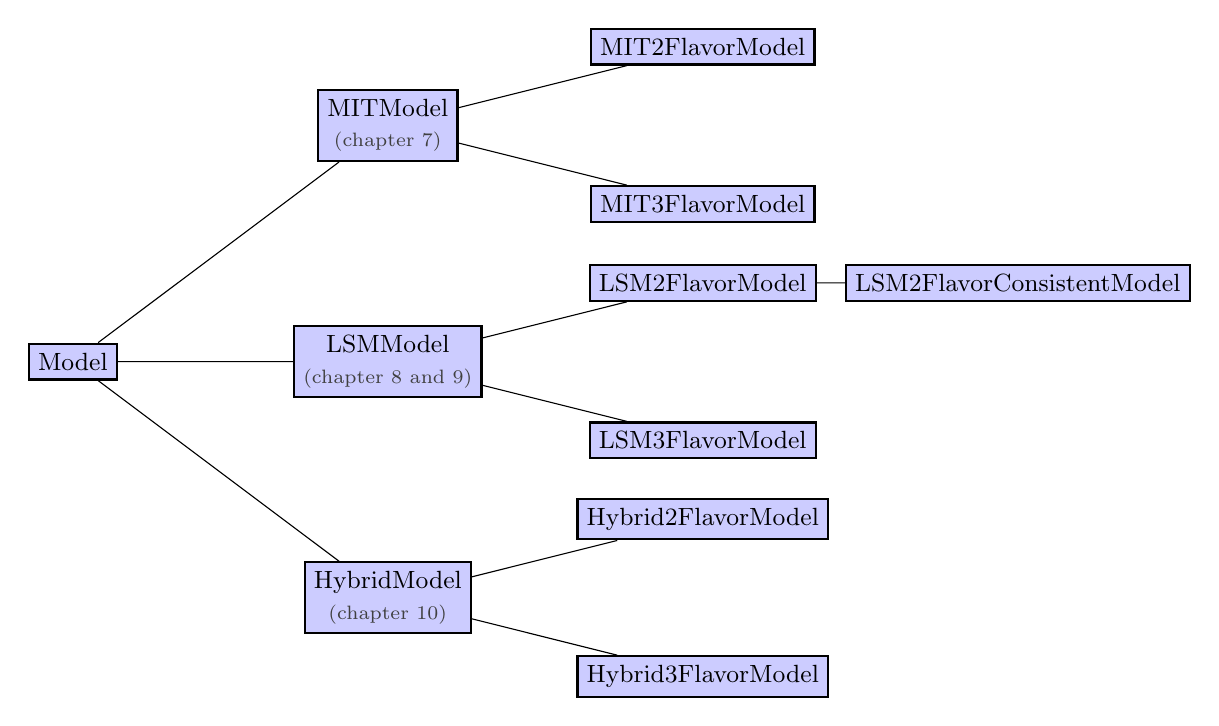
\begin{tikzpicture}[
	every node/.style={rectangle, fill=blue!20, draw=black, thick, font=\small, align=center}, % ellipse is too wide
	grow'=right,
	level distance=4cm,
	level 1/.style={sibling distance=3cm},
	level 2/.style={sibling distance=2cm},
]
\node {Model}
	child {node {MITModel \\ \scriptsize \textcolor{darkgray}{(chapter 7)}}
		child {node {MIT2FlavorModel}}
		child {node {MIT3FlavorModel}}
	}
	child {node {LSMModel \\ \scriptsize \textcolor{darkgray}{(chapter 8 and 9)}}
		child {node {LSM2FlavorModel}
			child {node {LSM2FlavorConsistentModel}}
		}
		child {node {LSM3FlavorModel}
			%child {node {LSM3FlavorAnomalyModel}}
		}
	}
	child {node {HybridModel \\ \scriptsize \textcolor{darkgray}{(chapter 10)}}
		child {node {Hybrid2FlavorModel}}
		child {node {Hybrid3FlavorModel}}
	};
\end{tikzpicture}
\end{center}

For each model, the program performs the following tasks:
\begin{itemize}
\item It numerically fits parameters to the grand potential \eqref{eq:master_intro:grand_potential} at zero temperature
      and evaluates it and its derivatives with respect to any mean fields that are present.
\item It finds the equation of state $\epsilon(P)$.
      First, pressures \eqref{eq:master_intro:pressure} and energy densities \eqref{eq:master_intro:energy_density} are parametrized with one independent mean field or chemical potential.
      Simultaneously, other mean fields and chemical potentials are determined by solving a system of equations that consist of the constraints \eqref{eq:lsm:chemical_equilibrium} and \eqref{eq:lsm:charge_neutrality} and self-consistency equations \eqref{eq:lsm:gap_equation} for any mean fields that are present.
      Finally, the independent variable is eliminated numerically to yield the equation of state.
      Numerically, the function $\epsilon(P)$ is implemented with splines as a linearly interpolating function between the parametrized points.
\item If the equation of state exhibits a phase transition,
      it is corrected with the Maxwell construction
      by establishing one vapor pressure at which the transition takes place,
      as explained in \cite[equation 4.69]{ref:master_francesco}.
\item It establishes upper or lower bounds for the bag constant $B$
      by making shifts \eqref{eq:mit:bag_shift} with different bag constants
      and solving the side of inequality \eqref{eq:mit:bag_stability} that matches the number of flavors in the model.
\item It integrates the Tolman-Oppenheimer-Volkoff equation \eqref{eq:master_intro:tov}
      using the program in \cref{sec:nstars:numtov},
      producing both mass-radius diagrams and radial profiles for various quantities in individual stars.
\end{itemize}

For readability, self-documentation and one-to-one correspondence,
the code uses Unicode variable names that resemble the variables and equations in the main text.

\codefile{python}{../code/quark_stars.py}{quark\_stars.py}
